% !TEX TS-program = lualatex
%---------%---------%
% pgfornament-doc.tex (utf8 encoding) - 简体中文译本
% Copyright 2012-2026  Alain Matthes
% SPDX-License-Identifier: LPPL-1.3c
% Maintainer: Alain Matthes
% 中文翻译：基于 pgfornament v1.4 (2026/10/17)
 \RequirePackage{luatex85}
% \RequirePackage{silence}
% \WarningsOff[latex]
% \WarningsOff[latexfont]
\documentclass[a4paper,nofonts]{tufte-handout}
%---------%---------%---------%---------%---------%---------%---------%---------
\usepackage{fontspec}
\setmainfont{texgyrepagella}%
[ Extension = .otf ,
  UprightFont = *-regular,
  ItalicFont = *-italic,
  BoldFont = *-bold,
  BoldItalicFont = *-bolditalic,
  Ligatures=TeX,
  Numbers={Lowercase,Monospaced}]
\setsansfont{texgyreheros}%
[ Extension = .otf,
  UprightFont = *-regular ,
  ItalicFont  = *-italic  ,
  BoldFont    = *-bold    ,
  BoldItalicFont = *-bolditalic]
\setmonofont{lmmono10-regular.otf}%
[ Numbers={Lining,SlashedZero},
  ItalicFont=lmmonoslant10-regular.otf,
  BoldFont=lmmonolt10-bold.otf,
  BoldItalicFont=lmmonolt10-boldoblique.otf]
\newfontfamily\ttcondensed{lmmonoltcond10-regular.otf}
 %% (La)TeX font-related declarations:
\linespread{1.05}% Pagella needs more space between lines
\frenchspacing
%---------%---------%---------%---------%---------%---------%---------%---------
% 中文支持：ctex 宏包（lualatex 环境）
\usepackage[UTF8]{ctex}
%---------%---------%---------%---------%---------%---------%---------%---------
\usepackage[dvipsnames,svgnames]{xcolor}
\usepackage{graphicx,rotating}
\usepackage[object=vectorian]{pgfornament}
\usetikzlibrary{chains,
                calc,
                scopes,
                decorations,
                decorations.text,
                decorations.markings,
                positioning,
                shapes.geometric}

\usepackage{tkzexample,tikzrput,pict2e,picture}

\usepackage{eso-pic,calc}
\usepackage{fancyvrb}
\usepackage{fourier}
\usepackage{amsmath,lipsum}  % extended mathematics
\usepackage{array,booktabs} % book-quality tables
\usepackage{multicol} % multiple column layout facilities
\usepackage{microtype}
\DisableLigatures{encoding = *, family = *}
% babel 已由 ctex 替代，不再单独加载
\setkeys{Gin}{width=\linewidth,totalheight=\textheight,keepaspectratio}
\graphicspath{{graphics/}} % set of paths to search for images
%\geometry{showframe} % display margins for debugging page layout
\fvset{fontsize=\small}
\hypersetup{%
pdfauthor = {Alain Matthes},
pdftitle = {pgfornament},
pdfsubject = {pgfornament 宏包文档（中文译本）},
colorlinks=true,
linkcolor=orange,
urlcolor=orange}

% section  (end)
%---------%---------%---------%---------%---------%---------%---------%---------
\title{pgfornament 装饰宏包}
\author{Alain Matthes}
\makeatletter
\AddToShipoutPicture{%
\begingroup 
\setlength{\@tempdima}{2mm}%
\setlength{\@tempdimb}{\paperwidth-\@tempdima-1cm}%
\setlength{\@tempdimc}{\paperheight-\@tempdima}%
\put(\LenToUnit{\@tempdima},\LenToUnit{\@tempdimc}){%
  \pgfornament[color=Maroon,anchor=north west,width=1cm]{39}}
\put(\LenToUnit{\@tempdimb},\LenToUnit{\@tempdimc}){%
  \pgfornament[color=Maroon,anchor=north east,width=1cm,symmetry=v]{39}} 
\put(\LenToUnit{\@tempdima},\LenToUnit{\@tempdima}){%
  \pgfornament[color=Maroon,anchor=south west,width=1cm,symmetry=h]{39}}
\put(\LenToUnit{\@tempdimb},\LenToUnit{\@tempdima}){%
  \pgfornament[color=Maroon,anchor=south east,width=1cm,symmetry=c]{39}}    
\endgroup  
} 
\let\strippt\strip@pt     
\makeatother
   
\newcommand{\eachpageornament}{%
\begin{picture}(0,0)
\put(0,0){\pgfornament[width=1cm]{41}};
\put(\strippt\textwidth,0){\pgfornament[width=1cm,symmetry=v]{41}};
\put(0,-\strippt\textheight){\pgfornament[width=1cm,symmetry=h]{41}};
\put(\strippt\textwidth,-\strippt\textheight){\pgfornament[width=1cm,symmetry=c]{41}};  %
\end{picture}}


% Standardize command font styles and environments
\newcommand{\docparen}[1]{\ensuremath{(#1)}}% optional command argument
\definecolor{fondpaille}{cmyk}{0,0,0.1,0}
\pagecolor{fondpaille}
\color{Maroon}
\colorlet{graphicbackground}{fondpaille}
\colorlet{numbackground}{fondpaille}
\colorlet{codebackground}{Periwinkle!10}
\colorlet{codeonlybackground}{Periwinkle!10}
\colorlet{textcodecolor}{MidnightBlue} % Maroon
\colorlet{numcolor}{gray}
\newcommand*{\tkzname}[1]{\textbf{\texttt{\textcolor{Maroon}{#1}}}}
\newcommand*{\PGF}{\tkzname{PGF}}
\newcommand*{\TIKZ}{\tkzname{Ti\emph{k}Z}}
\newcommand*{\pdf}{\textsc{pdf}}
\newcommand*{\pgfname}{\textsc{pgf}}
\newcommand*{\tikzname}{Ti\emph{k}Z}
\newcommand*{\pstricks}{\textsc{pstricks}}   %
\newcommand*{\tkzAttention}[3]{\ \\\llap{\textcolor{#3}{#1\hskip #2}}}
\newcommand*{\tkzHand}{\ \\\llap{\textcolor{red}{\lefthand\hskip1em}}}
\newcommand*{\tkzHandBomb}{\ \\\llap{\textcolor{red}{\lefthand\ \bomb\hskip1em}}}
\newcommand*{\tkzBomb}{\ \\\llap{\textcolor{red}{\bomb\hskip1em}}}
\newcommand*{\tkzTwoBomb}{\ \\\llap{\textcolor{red}{\bomb\ \bomb\hskip1em}}}
\newcommand*{\tkzimp}[1]{\textbf{#1}}
\newcommand*{\tkzcname}[1]{\textbf{\texttt{\textcolor{Maroon}{\textbackslash#1}}}}
\newcommand*{\tkzhname}[1]{\textbf{\texttt{\textcolor{Maroon}{\textbackslash#1}}}}
% Macros for typesetting the documentation
\newcommand{\hlred}[1]{\textcolor{Maroon}{#1}}% prints in red
\newcommand{\hangleft}[1]{\makebox[0pt][r]{#1}}
\newcommand{\hairsp}{\hspace{1pt}}% hair space
\newcommand{\hquad}{\hskip0.5em\relax}% half quad space
\newcommand{\TODO}{\textcolor{red}{\bf TODO!}\xspace}
\newcommand{\tuftebs}{\symbol{'134}}% a backslash in tt type in OT1/T1
\newcommand{\doccmdnoindex}[2][]{\texttt{\tuftebs#2}}% command name -- adds backslash automatically (and doesn't add cmd to the index)
\newcommand{\doccmddef}[2][]{%
  \hlred{\texttt{\tuftebs#2}}\label{cmd:#2}%
  \ifthenelse{\isempty{#1}}%
    {% add the command to the index
      \index{#2 command@\protect\hangleft{\texttt{\tuftebs}}\texttt{#2}}% command name
    }%
    {% add the command and package to the index
      \index{#2 command@\protect\hangleft{\texttt{\tuftebs}}\texttt{#2} (\texttt{#1} package)}% command name
      \index{#1 package@\texttt{#1} package}\index{packages!#1@\texttt{#1}}% package name
    }%
}% command name -- adds backslash automatically

\newcommand{\doccmd}[2][]{%
  \texttt{\tuftebs#2}%
  \ifthenelse{\isempty{#1}}%
    {% add the command to the index
      \index{#2 command@\protect\hangleft{\texttt{\tuftebs}}\texttt{#2}}% command name
    }%
    {% add the command and package to the index
      \index{#2 command@\protect\hangleft{\texttt{\tuftebs}}\texttt{#2} (\texttt{#1} package)}% command name
      \index{#1 package@\texttt{#1} package}\index{packages!#1@\texttt{#1}}% package name
    }%
}% command name -- adds backslash automatically
\newcommand{\docopt}[1]{\ensuremath{\protect\langle}\textrm{\textit{#1}}\ensuremath{\protect\rangle}}% optional command argument
\newcommand{\docarg}[1]{\textrm{\textit{#1}}}% (required) command argument
\newenvironment{docspec}{\begin{quotation}\ttfamily\parskip0pt\parindent0pt\ignorespaces}{\end{quotation}}% command specification environment
\newcommand{\docdist}[1]{\texttt{#1}\index{#1 distribution@\texttt{#1} distribution}\index{distributions!#1@\texttt{#1}}}% environment name
\newcommand{\docenv}[1]{\texttt{#1}\index{#1 environment@\texttt{#1} environment}\index{environments!#1@\texttt{#1}}}% environment name
\newcommand{\docenvdef}[1]{\hlred{\texttt{#1}}\label{env:#1}\index{#1 environment@\texttt{#1} environment}\index{environments!#1@\texttt{#1}}}% environment name
\newcommand{\docoption}[2]{\texttt{#1}\index{#1 option@\texttt{#1} option}\index{options(#2)!#1@\texttt{#1}}}% package name
\newcommand{\docpkg}[1]{\texttt{#1}\index{#1 package@\texttt{#1} package}\index{packages!#1@\texttt{#1}}}% package name
\newcommand{\doclib}[1]{\texttt{#1}\index{#1 tikz library@\texttt{#1} library}\index{library!#1@\texttt{#1}}}% libray name
\newcommand{\doccls}[1]{\texttt{#1}}% document class name
\newcommand{\docclsopt}[1]{\texttt{#1}\index{#1 class option@\texttt{#1} class option}\index{class options!#1@\texttt{#1}}}% document class option name
\newcommand{\docclsoptdef}[1]{\hlred{\texttt{#1}}\label{clsopt:#1}\index{#1 class option@\texttt{#1} class option}\index{class options!#1@\texttt{#1}}}% document class option name defined
\newcommand{\docmsg}[2]{\bigskip\begin{fullwidth}
\noindent\ttfamily#1\end{fullwidth}\medskip\par\noindent#2}
\newcommand{\docfilehook}[2]{\texttt{#1}\index{file hooks!#2}\index{#1@\texttt{#1}}}
\newcommand{\doccounter}[1]{\texttt{#1}\index{#1 counter@\texttt{#1} counter}}
\newcommand{\docStyle}[1]{\texttt{#1}\index{#1 style(\TIKZ)@\texttt{#1} style(\TIKZ)}\index{styles(\TIKZ)!#1@\texttt{#1}}}% package name
\newcommand*{\Imacro}[1]{\index{#1_1@\texttt{\textbackslash#1}}}%n
\newcommand{\docfamily}[1]{\texttt{#1}\index{#1 family@\texttt{#1} family}\index{families!#1@\texttt{#1}}}% package name
\newcommand{\docvo}[1]{\texttt{#1}\index{#1 vector ornament@\texttt{#1} vector ornament}\index{vector ornaments!#1@\texttt{#1}}}% package name
%


\endinput
\usepackage{makeidx}
\makeindex
\renewenvironment{theindex}
  {\renewcommand\item{\par\hangindent 40pt}
   \renewcommand\subitem{\item\hspace*{20pt}}
   \renewcommand\subsubitem{\item\hspace*{30pt}}
   \renewcommand\indexspace{\par \vskip 10pt plus 5pt minus 3pt\relax}
   \section{\indexname}
   \begin{multicols}{2}%
    \parindent=0pt
     \small%
      }
  {\end{multicols}%
  }

\makeatletter
\newcommand{\getpgfornamentDim}[1]{%
 {\@pgfornamentDim{#1}%
 X:~\@pgfornamentX\\Y:~\@pgfornamentY}%
}
\newcommand{\adjustpgfornamentDim}[1]{%
\@pgfornamentDim{#1}%
\pgfmathsetmacro{\pgfcoeff}{\@pgfornamentX/\@pgfornamentY}%
}
\makeatother

\newcommand{\ornamentview}[1]{%
\foreach \n in {#1} {%
\begin{tikzpicture}
  \adjustpgfornamentDim{\n}
  \ifdim\pgfcoeff pt >1 pt \relax \def\adjustXY{2}
  \else
  \pgfmathsetmacro{\adjustXY}{2*\pgfcoeff}
  \fi
\draw[Maroon](-1.25cm,-1.25cm) rectangle (1.25cm,1.25cm);
\node[inner sep=0pt] (element) {\pgfornament[width=\adjustXY cm]{\n}};
\node[anchor=north west,inner sep=0pt,font=\small\bfseries\sffamily,color=red] at (2.05cm,1.05cm) {\n};
\node[anchor=west,text width=4em,font=\footnotesize] at (1.85cm,0) {\getpgfornamentDim{\n}};
\end{tikzpicture}%
\space\space\space\space}}%

%---------%---------%---------%---------%---------%---------%---------%---------
%---------%---------%---------%---------%---------%---------%---------%---------
\begin{document}

\maketitle
\noindent\pgfornament[symmetry=c,width=2cm]{46}
\begin{marginfigure}
  
\begin{tikzpicture}[baseline={(current bounding box.center)}] \tikzset{pgfornamentstyle/.style={
  draw=Goldenrod,fill=Red,line width=1pt}}
  \node[fill=black,circle,draw=Red,line width=2pt,inner sep=8pt]
  at (0,0) {\pgfornament[scale=0.38]{56}};
  \end{tikzpicture}
\end{marginfigure}


\bigskip
\noindent\pgfornament[width=0.75 cm]{152}\ （版本 1.4，2026/10/17）
\begin{abstract}

本文档介绍 \LaTeX\ 宏包 \emph{\docpkg{pgfornament}}，阐述宏 \texttt{pgfornament} 的语法与参数，并提供该宏包使用示例与说明。

首先，我要感谢 {Till \textsc{Tantau}} 开发了如此精美的 \LaTeX\ 宏包——\TIKZ。

感谢 Vincent \textsc{Le Moign} 允许我们以 Pstricks 和 \PGF/\TIKZ 格式分发这些装饰纹样\sidenote{ \url{http://www.vectorian.net/}（免费样本）}。

同时感谢 \textsc{P. Fradin}，他最早为 PStricks 创建了装饰纹样宏包，这启发我在 \TIKZ 上做同样的工作。

还要感谢 {Enrico \textsc{Gregorio}}，本宏包中的一些出色创意正源自他。您将在本文档末尾找到宏包附带的 196 个符号。

在新版本中，我们加入了一组新的装饰纹样。\textsc{Chennan Zhang} 使用 CAD 软件绘制了这些纹样，再用 TikZ 重新绘制，并授权 \textsc{LianTze Lim} 将其整理为库（\emph{\docpkg{pgfornament-han}}），以供 pgfornament 宏包使用。现在可以直接使用中国传统纹样与图案库了。

除本文档外，您还可参阅 \emph{\docpkg{tikzrput}} 宏包的相关文档。
\end{abstract}

%---------%---------%---------%---------%---------%---------%---------%---------
\vspace{1cm}
\hfil  \pgfornament[width=4cm]{84}\hfil

\tableofcontents

\vspace{1cm}
\hfil  \pgfornament[width=4cm]{84}\hfil

\listoffigures

\vspace{1cm}
\hfil  \pgfornament[width=4cm]{84}\hfil


\section{如何安装宏包}
\label{sec:how_to_install}
对于 \docdist{TeXLive}，如果你需要自行安装，宏包提供了符合 TDS 规范的 zip 压缩包（pgfornament.zip）。
只需下载该文件，并将其解压到你的 TDS 目录中（类 Unix 系统为 \texttt{~/texmf}）。
\begin{itemize}
  \item \docpkg{pgfornament} 必须放置在 \texttt{~/texmf/tex/latex}
  \item 各库文件 \texttt{pgfornament-lib-vectorian.code.tex}、\texttt{pgfornament-lib-pgfhan.code.tex}、
        \texttt{pgfornament-lib-celtic.code.tex} 和 \texttt{pgfornament-lib-am.code.tex} 必须放置在 \texttt{~/texmf/tex/latex}
  \item 目录 vectorian、pgfhan、celtic 和 am（即文件 \texttt{pgfornament-vectorian1.pgf} 等）必须放置在 \texttt{~/texmf/tex/generic}
\end{itemize}

对于 \docdist{MiKTeX}，将目录 {\color{black}\texttt{pgfornament}} 复制到 \verb+C:\texmf\tex\latex+，然后
运行 {\color{red}\texttt{MiKTeX 选项}}。在 {\color{black}\texttt{文件名数据库}} 栏目中，点击 {\color{red}\texttt{立即刷新}}。

\section{如何使用宏包}
\label{sec:how_to_use}
你只需在导言区添加 \\
{\color{black}\verb+\usepackage{pgfornament}+} \\ 或 \\{\color{black}\verb+\usepackage[object=vectorian]{pgfornament}+}\\
即可。pgfornament 宏包会自动加载 \TIKZ。

若不指定任何选项，pgfornament 宏包默认使用 \docfamily{vectorian} 纹样。如果你想使用其他纹样集，可按如下方式指定纹样列表名称：\\
{\color{black}\verb+\usepackage[object=pgfhan]{pgfornament}+}.\\
\docfamily{pgfhan} 是中国传统纹样与图案集。
\docfamily{celtic} 是凯尔特结纹样集（公共领域，参见第 \ref{sec:celtic} 节）。

我创建了 \docfamily{am} 示例集，用于演示如何创建新纹样以及如何使用它（参见第 \ref{am1def} 节）。
下面是获取矢量装饰纹样的最小代码示例。
\colorlet{graphicbackground}{blue!10!white}%
\colorlet{codebackground}{red!10}%

\begin{marginfigure}%
\begin{center}
  \pgfornament[width = 2cm,
               color = red]{1}
\end{center}
\caption{最小代码的运行结果}
\end{marginfigure}

\begin{tkzexample}[code only,very small]
 \documentclass{scrartcl}
 \usepackage{pgfornament}
 \begin{document}
 \pgfornament[width = 2cm,
              color = red]{1}
 \end{document}
\end{tkzexample}

如果你想使用 Han 纹样库

\newpgfornamentfamily{pgfhan}
\begin{marginfigure}%
\begin{center}
  \pgfornament[width = 2cm,
               color = SeaGreen]{78}
\end{center}
\caption{最小代码的运行结果}
\end{marginfigure}

\begin{tkzexample}[code only,very small]
 \documentclass{scrartcl}
 \usepackage[object=pgfhan]{pgfornament}
 \begin{document}
 \pgfornament[width = 2cm,
              color = SeaGreen]{78}
 \end{document}
\end{tkzexample}
\newpgfornamentfamily{vectorian}

如何使用不同的装饰纹样集？

有两种方式：使用宏 \doccmd{newpgfornamentfamily}，或者使用环境 \docenv{newfamily}

例如：
\newpgfornamentfamily{pgfhan}
\pgfornament[width = 2cm, color = SeaGreen]{59}
\newpgfornamentfamily{vectorian}
\pgfornament[width = 2cm, color = SeaGreen]{59}

对应代码如下：
\begin{tkzexample}[code only, very small]
  \newpgfornamentfamily{pgfhan}
  \pgfornament[width = 2cm, color = SeaGreen]{59}
  \newpgfornamentfamily{vectorian}
  \pgfornament[width = 2cm, color = SeaGreen]{59}
\end{tkzexample}

下面使用环境方式。结束后，纹样库会恢复为之前的设置。

\begin{newfamily}[pgfhan]
  
\begin{tikzpicture}
  \node{ \pgfornament[color=Dandelion,width=2cm]{1}};
  \end{tikzpicture}
\end{newfamily}


\begin{tikzpicture}
\node{\pgfornament[color=MidnightBlue,width=2cm]{1}};
\end{tikzpicture}

对应代码如下：
\begin{tkzexample}[code only, very small]
\begin{newfamily}[pgfhan]
  
\begin{tikzpicture}
  \node{ \pgfornament[color=Dandelion,width=2cm]{1}};
  \end{tikzpicture}
\end{newfamily}


\begin{tikzpicture}
\node{\pgfornament[color=MidnightBlue,width=2cm]{1}};
\end{tikzpicture}
\end{tkzexample}

\section{主宏}
\label{sec:the_main_macro}

宏 \doccmd{pgfornament} 用于绘制与指定编号对应的纹样。对于 vectorian 纹样集，编号范围为 $1$ 至 $196$。该宏可以独立使用，也可以放在图形环境中调用。它本质上是一个放置在当前位置的 \emph{\docenv{tikzpicture}} 环境。

显示的纹样取决于调用 \doccmd{pgfornament} 时所使用的选项。
{\color{red}\Verb|\pgfornament|} 命令的语法说明如下：
\begin{docspec}
 \color{black} \doccmd{pgfornament[\docopt{options}]\{\docarg{number}\}}
\end{docspec}

输出结果是一幅由 \emph{\docenv{tikzpicture}} 环境定义的图形。

\subsection{数字参数}
\label{sub:arg_number}

数字参数用于按序号指定纹样列表中的某一项。
\begin{marginfigure}
\begin{center}
  \pgfornament[width=2cm,color=RubineRed]{1}
\end{center}
\caption{Vectorian 装饰纹样编号 1}
\end{marginfigure}
\begin{tkzexample}[code only,width=5cm,very small]
  \usepackage{pgfornament}
  ...
  \pgfornament[width=2cm]{1}
\end{tkzexample}

\medskip
\begin{marginfigure}
\begin{center}
  \pgfornament[width=2cm,color=SeaGreen]{2}
\end{center}
  \caption{Vectorian 装饰纹样编号 2}
\end{marginfigure}
\begin{tkzexample}[code only,width=5cm,very small]
  \usepackage{pgfornament}
  ...
  \pgfornament[width=2cm]{2}
\end{tkzexample}

\medskip
\begin{marginfigure}
\begin{center}
\begin{newfamily}[pgfhan]

\begin{tikzpicture}
 \node {\pgfornament[color=red,width=2cm]{57}};
\end{tikzpicture}
\end{newfamily}
\end{center}
\caption{中式装饰纹样编号 57}
\end{marginfigure}
\begin{tkzexample}[code only,width=5cm,very small]
  \usepackage[object=pgfhan]{pgfornament}
    ...
  \pgfornament[color=Mahogany,width=2cm]{57}
\end{tkzexample}

\medskip
\begin{tkzexample}[code only,width=5cm,very small]
  \usepackage[object=am]{pgfornament}
   ...
  \pgfornament[width=4cm]{1}
\end{tkzexample}
\begin{marginfigure}
\begin{newfamily}[am]

\begin{tikzpicture}
 \pgfornament[color=Dandelion,width=2cm]{1}
\end{tikzpicture}
\end{newfamily}
\newpgfornamentfamily{vectorian}
  \caption{am 装饰纹样编号 1}
\end{marginfigure}

\subsection{参数与选项}
\label{sub:the_options}
该宏共有六个选项。其中 \Verb+symmetry+ 选项有四种取值。
下表详细说明这些选项。

\begin{table}[h]\index{pgfornament!options}
{ \small   \begin{tabular}{lll}
      \toprule
 名称 & 默认值 & 说明 \\
\midrule
\docoption{scale}{pgfornament}         & 1     & 高宽比保持不变\\
\docoption{width}{pgfornament}         & \{\}  & 设置宽度，比例不变  \\
\docoption{height}{pgfornament}        & \{\}  & 设置高度，比例不变 \\
\docoption{color}{pgfornament}         & black & 装饰纹样的颜色  \\
\docoption{opacity}{pgfornament}       & 1     & 不超过 1 的数值，装饰纹样的不透明度  \\
\docoption{ydelta}{pgfornament}        & 0 pt  & 用于垂直方向微调装饰纹样的数值  \\
\docoption{symmetry=v}{pgfornament}    & none  &  垂直镜像对称\\
\docoption{symmetry=h}{pgfornament}    & none  & 水平镜像对称 \\
\docoption{symmetry=c}{pgfornament}    & none  & 中心对称 \\
\docoption{symmetry=none}{pgfornament} & none  & 默认无对称效果 \\
\bottomrule
\end{tabular} }
\caption{pgfornament 宏的选项列表。}
  \label{tab:pgfornament-options}
\end{table}

\subsection{选项使用示例}
\label{sub:examples}
\begin{enumerate}\setlength{\itemsep}{30pt}
\item 选项 \docoption{scale}{pgfornament}
\begin{tkzexample}[code only,very small]
  \pgfornament[scale=0.25]{77}
\end{tkzexample}
\begin{marginfigure}
  \pgfornament[scale=0.25]{77}
\caption{选项 \tkzname{scale}}
\end{marginfigure}
\item 选项 \docoption{width}{pgfornament}
\begin{tkzexample}[code only,very small]
 \pgfornament[width=5cm]{77}
\end{tkzexample}
\begin{marginfigure}
  \pgfornament[width=5cm]{77}
\caption{选项 \tkzname{width}}
\end{marginfigure}
\item 选项 \docoption{height}{pgfornament}
\begin{tkzexample}[code only,very small]
\pgfornament[height=1cm]{77}
\end{tkzexample}
\begin{marginfigure}
  \pgfornament[height=1cm]{77}
\caption{选项 \tkzname{height}}
\end{marginfigure}

\item 选项 \docoption{color}{pgfornament}
\begin{tkzexample}[code only,very small]
\pgfornament[height=1cm,color=green!20!black]{77}
\end{tkzexample}
\begin{marginfigure}
\pgfornament[height=1cm,color=green!20!black]{77}
\caption{选项 \tkzname{color}}
\end{marginfigure}


\begin{marginfigure}
  \pgfornament[color=MidnightBlue,width=3cm]{24}%
  \caption{如何使用 \tkzname{color}}
\end{marginfigure}
\begin{tkzexample}[code only,very small]
  \pgfornament[color=MidnightBlue,width=3cm]{24}%
\end{tkzexample}

\item 选项 \docoption{opacity}{pgfornament}
\begin{tkzexample}[code only,very small]
\pgfornament[height=1cm,color=green!20!black,opacity=0.2]{77}
\end{tkzexample}
\begin{marginfigure}
\pgfornament[height=1cm,color=green!20!black,opacity=0.2]{77}
\caption{选项 \tkzname{opacity}}
\end{marginfigure}

\begin{marginfigure}
  \pgfornament[width=5cm]{2}
      \caption{对称效果示例}
\end{marginfigure}

\item 选项 \docoption{symmetry=h}{pgfornament}
（水平轴对称）
\begin{marginfigure}
 \tikzset{pgfornamentstyle/.style={draw=BlueGreen,
             fill=BlueGreen!20,fill opacity=.5,thick}}%
\pgfornament[width=5cm,symmetry=h]{2}
\caption{水平对称}
\end{marginfigure}


\item 选项 \docoption{symmetry=v}{pgfornament}
（垂直轴对称）
\begin{marginfigure}
\tikzset{pgfornamentstyle/.style={draw=MidnightBlue,
        fill=MidnightBlue!20,fill opacity=.5,thick}}%
\pgfornament[width=5cm,symmetry=v]{2}
\caption{垂直对称}
\end{marginfigure}

\item 选项 \docoption{symmetry=c}{pgfornament}
（关于原点中心对称）
\begin{marginfigure}
\tikzset{pgfornamentstyle/.style={draw=RubineRed,
           fill=RubineRed!20,fill opacity=.5,thick}}%
\pgfornament[width=5cm,symmetry=c]{2}%
\caption{中心对称}
\end{marginfigure}

\item 选项 \docoption{ydelta}{pgfornament}

\begin{marginfigure}%
\pgfornament[color=MidnightBlue,width=1cm,ydelta=-10pt]{25}%
\pgfornament[color=PineGreen,width=1cm]{25}%
\pgfornament[color=Periwinkle,width=1cm,ydelta=+10pt]{25}%
\caption{如何使用 \tkzname{ydelta}}
\end{marginfigure}
\begin{tkzexample}[code only,very small]
  \pgfornament[color=MidnightBlue,width=2cm,ydelta=-10pt]{25}%
  \pgfornament[color=PineGreen,width=2cm]{25}%
  \pgfornament[color=Periwinkle,width=2cm,ydelta=+10pt]{25}%
\end{tkzexample}
\end{enumerate}

\clearpage\newpage
\subsection{样式 \docStyle{pgfornamentstyle}}
\label{sub:pgfornamentstyle}
该样式可用于修改颜色等选项，以及在可行时设置纹样的填充方式。
\begin{marginfigure}%

\begin{tikzpicture}
  \tikzset{pgfornamentstyle/.style={
           fill=SpringGreen,
           fill opacity=.5,
           line width=1pt}}%
  \pgfornament[color=OliveGreen,scale=1.25,anchor=south]{24}%
\end{tikzpicture}
\caption{如何使用样式 \tkzname{pgfornamentstyle}}
\end{marginfigure}
\begin{tkzexample}[code only,very small]

\begin{tikzpicture}
  \tikzset{pgfornamentstyle/.style={
           fill=SpringGreen,
           fill opacity=.5,
           line width=1pt}}%
  \pgfornament[color=OliveGreen,scale=1.25,anchor=south]{24}%
\end{tikzpicture}
\end{tkzexample}

\subsection{来自 \docpkg{\TIKZ} 的高级选项}
\label{sub:advanced_options}
\begin{marginfigure}

\begin{tikzpicture}
 \tikzset{pgfornamentstyle/.style={draw=Periwinkle,
             fill=SpringGreen}}%
 \node[draw=Periwinkle,circle,anchor=center,
      inner sep=0pt,fill=GreenYellow] at (0,0){%
\pgfornament[anchor=center]{24}};
\end{tikzpicture}
\caption{如何添加 \TIKZ 样式}
\end{marginfigure}
\begin{tkzexample}[code only,very small]

\begin{tikzpicture}
 \tikzset{pgfornamentstyle/.style={draw=Periwinkle,
             fill=SpringGreen}}%
 \node[draw=Periwinkle,circle,anchor=center,
      inner sep=0pt,fill=GreenYellow] at (0,0){%
 \pgfornament[anchor=center]{24}};
\end{tikzpicture}
\end{tkzexample}

\section{什么是（pgf）装饰纹样？}
\label{sec:what_is_a_pgf_ornament}
当你在文档中写入 \Verb|\pgfornament{1}| 时，就会得到某一族中的第一个装饰纹样（默认是 \docfamily{vectorian} 族）。该纹样是一个矢量对象，由 \emph{\docenv{tikzpicture}} 环境定义。
\begin{tkzexample}[code only,very small]
\begin{tikzpicture}[baseline={([yshift=\pgfornamentydelta]%
  current bounding box.\pgfornamentanchor)},pgfornamentstyle]
  \pgftransformscale{\pgfornamentscale}%
  \pgf@@ornament{#2}%
\end{tikzpicture}%
\end{tkzexample}

\medskip
你可以通过修改 \doccmd{pgfornamentscale} 或 \docStyle{pgfornamentstyle} 来改变图形的外观。使用 \doccmd{pgfornamentydelta} 或 \doccmd{pgfornamentanchor} 可以移动图形，但具体效果取决于不同的使用环境。下面的代码给出了图 \ref{fig:minimum} 所示的图形。我选择这种方法是为了让使用尽可能简单。
\begin{marginfigure}
 \pgfornament[anchor=center,scale=1]{1}
 \caption{得到一个装饰纹样的最简代码}
 \label{fig:minimum}
\end{marginfigure}
\begin{tkzexample}[code only,very small]
 \documentclass{scrartcl}
 \usepackage{pgfornament}
 \begin{document}
 \pgfornament{1}
 \end{document}
\end{tkzexample}

\medskip
装饰纹样被放置在一个矩形区域内\sidenote{你可以在文件 pgfornament-lib-vectorian.code.tex 中找到该形状的尺寸。该文件名取决于矢量族的名称，默认情况下是 \docfamily{vectorian}。}。

\medskip
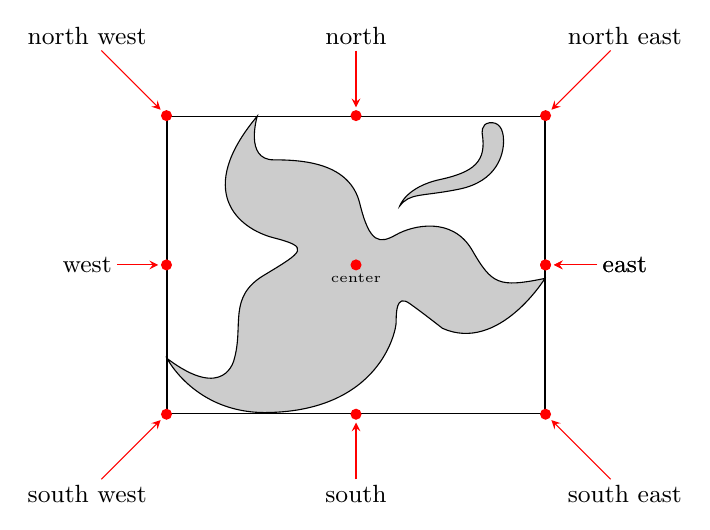
\begin{tikzpicture}[every node/.style={inner sep=0pt}]
  \tikzset{image/.style={circle,
                         fill=red,
                         minimum size = 4pt,
                         inner sep    = 0pt,
                         outer sep    = 1pt}
                         }

\node[inner sep = 1cm] (wrapper){\tikz
\node[draw](image) {\pgfsetfillopacity{0.2}\pgfornament{1}};};

\foreach \ancre  in {north,north east,east,south east,south,south west,west,north west,east}
{%
 \node [image] (i\ancre) at (image.\ancre) {};
 \node [outer sep=2pt] (w\ancre) at (wrapper.\ancre) {\small\ancre};
 \draw [red,->,>=stealth] (w\ancre)--(i\ancre);
 }
 \node[image,label=below:{\tiny center}] at (wrapper.center) {};
\end{tikzpicture}

在上图中，我标出了你可以使用的所有锚点 \index{anchors}。接下来你将看到如何把这个图形放置在页面上、文本流中，或是一个复杂图形的内部。

\section{在页面上放置矢量装饰纹样}
\label{sec:placement_on_a_page}

\unitlength=1pt
\noindent\eachpageornament
\subsection{借助 \docpkg{eso-pic} 宏包在每页放置}
\label{sub:with_the_package_eso_pic}

你可能已经注意到每页的四个角都放置了装饰纹样。下面的代码说明了如何实现这一点。代码中与 \docpkg{pgfornament} 相关的部分仅仅是使用了 \doccmd{pgfornament} 这个宏。为了把对象准确地放置在页面上的合适位置，我们需要考虑它的宽度。

也许你已经注意到了每页四角的装饰纹样

我使用了 \docpkg{eso-pic} 宏包以及下面的代码。宏 \doccmd{put} 把装饰纹样放置在某个点上，但你需要正确地设置锚点。

\begin{tkzexample}[code only,very small]
\usepackage{eso-pic}
\makeatletter
\AddToShipoutPicture{%
\begingroup
\setlength{\@tempdima}{2mm}%
\setlength{\@tempdimb}{\paperwidth-\@tempdima-2cm}%
\setlength{\@tempdimc}{\paperheight-\@tempdima}%
\put(\LenToUnit{\@tempdima},\LenToUnit{\@tempdimc}){%
 \pgfornament[anchor=north west,width=2cm]{63}}
\put(\LenToUnit{\@tempdima},\LenToUnit{\@tempdima}){%
  \pgfornament[anchor=south west,width=2cm,symmetry=h]{63}}
\put(\LenToUnit{\@tempdimb},\LenToUnit{\@tempdimc}){%
  \pgfornament[anchor=north east,width=2cm,symmetry=v]{63}}
\put(\LenToUnit{\@tempdimb},\LenToUnit{\@tempdima}){%
  \pgfornament[anchor=south east,width=2cm,symmetry=c]{63}}
\endgroup
}
\makeatother
\end{tkzexample}
\Imacro{AddToShipoutPicture}  \Imacro{LenToUnit}  \Imacro{anchor}

\subsection{借助 picture 环境在单页放置}
\label{sub:with_the_picture_environment}

下面的代码用于在 tufte 文档类所定义的页面上划定文本区域。
\sidenote{\tkzcname{strippt} 由 \tkzcname{let}\doccmd{strippt}\doccmd{strip@pt} 定义}
\begin{tkzexample}[code only,very small]
\newcommand{\eachpageornament}{%
\unitlength=1pt
\begin{picture}(0,0)%
\put(0,0){\pgfornament[width=1cm]{41}};%
\put(\strippt\textwidth,0){%
     \pgfornament[width=1cm,symmetry=v]{41}};%
\put(0,-\strippt\textheight){%
      \pgfornament[width=1cm,symmetry=h]{41}};%
\put(\strippt\textwidth,-\strippt\textheight){%
      \pgfornament[width=1cm,symmetry=c]{41}};%
\end{picture}}%

\eachpageornament
\end{tkzexample}

\subsection{使用 \docpkg{\TIKZ} 的 \tkzname{remember picture} 与 \tkzname{overlay}}
\label{sub:with_tikz}

你可以不使用 \docpkg{eso-pic}，而是借助 \docpkg{\TIKZ}\ 并通过下面的宏在单页上得到相同的效果。\tkzname{remember picture} 是必需的，该选项告诉 \TIKZ\ 应尝试记住当前图形在页面上的位置，使用此类代码时你需要编译两次。选项 \tkzname{overlay}\index{overlay}\ 会切换包围盒的计算方式，从而使图形不进入文本流，也不会改变版面布局。

\begin{tkzexample}[code only,very small]
\newcommand{\eachpageornament}{%
\begin{tikzpicture}[remember picture, overlay]
    \node[anchor=north west] at (current page.north west){%
                      \pgfornament[width=2cm]{63}};
    \node[anchor=north east] at (current page.north east){%
                      \pgfornament[width=2cm,symmetry=v]{63}};
    \node[anchor=south west] at (current page.south west){%
                     \pgfornament[width=2cm,symmetry=h]{63}};
    \node[anchor=south east] at (current page.south east){%
                      \pgfornament[width=2cm,symmetry=c]{63}};
\end{tikzpicture}
}
\end{tkzexample}
\index{current page}

\section{在文本流中放置矢量装饰纹样}
\label{sec:placing-ornament}
\subsection{\protect\pgfornament[anchor=south,width=1cm]{78}\  直接放置 \  \protect\pgfornament[anchor=south,width=1cm,symmetry=v]{78}}
\label{sub:directly}

下面的代码向你展示选择不同锚点所产生的效果。
\setlength{\fboxsep}{0pt}

{\color{black}基线
\pgfsetfillopacity{0.2}%
\fbox{\pgfornament[anchor=south,width=2cm]{69}}%
\fbox{\pgfornament[width=2cm]{69}}%
\fbox{\pgfornament[anchor=north,width=2cm]{69}}%
\pgfsetfillopacity{1} 基线 }

\begin{tkzexample}[code only,very small]
{ \color{black}baseline \pgfsetfillopacity{0.2}%
  \fbox{\pgfornament[anchor=south,width=2cm]{69}}%
  \fbox{\pgfornament[width=2cm]{69}}%
  \fbox{\pgfornament[anchor=north,width=2cm]{69}}%
  \pgfsetfillopacity{1} baseline }
\end{tkzexample}

\medskip
\noindent 也许你会对修改小节标题所用的代码感兴趣？

\begin{tkzexample}[code only,very small]
\subsection{\protect\pgfornament[anchor=south,width=1cm]{78}\
    Directly \
    \protect\pgfornament[anchor=south,width=1cm,symmetry=v]{78}}
\end{tkzexample}

\subsection{在 \TIKZ 文本流中放置}
\label{sub:in_the_flow_with_tikz}

\medskip
一般来说，最好的做法是把装饰纹样放在一个节点中，再把节点放在一个 \emph{tikzpicture} 环境里。你可以指定节点在 \emph{\docenv{tikzpicture}} 中的位置，也可以添加锚点来按你想要的方式精确放置装饰纹样。

\begin{marginfigure}
  \begin{center}
    
\begin{tikzpicture}
      \foreach \a in {0,45,...,315}
     \node[anchor=west,rotate=\a,inner sep=0pt,xshift=12pt] {%
     \pgfornament[width=1cm]{88}};
    \end{tikzpicture}
  \end{center}
  \caption{装饰纹样的组合（版本 2）}
\end{marginfigure}

\begin{tkzexample}[code only,very small]

\begin{tikzpicture}
    \foreach \a in {0,45,...,315}
      \node[anchor=west,rotate=\a,inner sep=0pt,xshift=12pt] {%
      \pgfornament[width=1cm]{88}};
\end{tikzpicture}
\end{tkzexample}

\begin{marginfigure}
  \begin{center}
    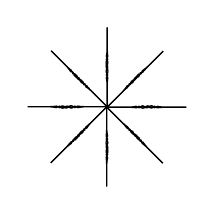
\begin{tikzpicture}
      \foreach \a in {0,45,...,315}
        \node[anchor=west,rotate=\a,inner sep=0pt] {%
     \pgfornament[width=1cm]{88}};
    \end{tikzpicture}
  \end{center}
  \caption{装饰纹样的组合（版本 1）}
\end{marginfigure}

\begin{tkzexample}[code only,very small]
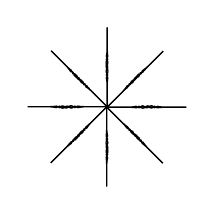
\begin{tikzpicture}
    \foreach \a in {0,45,...,315}
      \node[anchor=west,rotate=\a,inner sep=0pt] {%
      \pgfornament[width=1cm]{88}};
\end{tikzpicture}
\end{tkzexample}

\medskip
\emph{注意：使用 \emph{\doccmd{put}} 和 \emph{\doccmd{rotatebox}} 很难得到相同的效果，但借助 \emph{\docpkg{rotating}} 宏包则很容易。}

\begin{marginfigure}
  \begin{center}
\foreach \a in {0,45,...,315}{%
   \turnbox{\a}{\pgfornament[width=1cm]{88}}}%
  \end{center}
\end{marginfigure}

\begin{tkzexample}[code only,very small]
  \foreach \a in {0,45,...,315}{%
     \turnbox{\a}{\pgfornament[width=1cm]{88}}}%
\end{tkzexample}

\section{在节点内部放置装饰纹样}
\label{sec:inside}
这种方法非常实用且灵活，因为可以通过 \doccmd{node} 命令使用各种选项和样式。你可以修改 \docoption{pgfornamentstyle}{pgfornament} 的样式\sidenote{如果你想恢复默认样式，可以使用 \doccmd{resetpgfornamentstyle}。}。

\begin{marginfigure}
\tikzset{pgfornamentstyle/.style={draw=green!20!black,inner sep=0pt,
           fill=orange,fill opacity=.5,scale=1.25,ultra thick}}%
\tikz\node {\fbox{\pgfornament{3}}};
\caption{配合节点使用样式}
\end{marginfigure}
\begin{tkzexample}[code only,very small]
\tikzset{pgfornamentstyle/.style={%
  draw=green!20!black,inner sep=0pt,fill=orange,
  fill opacity=.5,scale=1.25,ultra thick}}%
  \tikz\node {\fbox{\pgfornament{3}}};
\end{tkzexample}



{\textcolor{red}{\pgfornament[width=0.5 cm]{152} \hskip1em}} 如果我们在文本流中使用 tikzpicture，那么了解如何放置该图形就非常有用。代码中的关键部分是：\\

\begin{tkzexample}[code only,very small]
  \tikz[baseline=(current bounding box.south)]
\end{tkzexample}  \index{current bounding box}

 \medskip
{\textcolor{red}{\pgfornament[width=0.5 cm]{152}} 不要忘记使用 \tkzname{inner sep =0pt}\index{inner sep}，否则对象周围可能会出现多余的空隙。}\\

\begin{tkzexample}[code only,very small]
baseline\tikz[baseline]
\node[inner sep=0pt]{\fbox{\pgfornament[width=2cm]{3}}};
baseline
\tikz[baseline=(current bounding box.south)]
\node[inner sep=0pt]{\fbox{\pgfornament[width=2cm]{3}}};
baseline
\tikz[baseline=(current bounding box.north)]
\node[inner sep=0pt]{\fbox{\pgfornament[width=2cm]{3}}};
baseline
\end{tkzexample} \index{baseline}

\begin{figure}
  baseline\tikz[baseline]\node[inner sep=0pt] {\fbox{\pgfornament[width=1.5cm]{3}}};%
  baseline\tikz[baseline=(current bounding box.south)]\node[inner sep=0pt] {\fbox{\pgfornament[width=1.5cm]{3}}};%
  baseline\tikz[baseline=(current bounding box.north)]\node[inner sep=0pt] {\fbox{\pgfornament[width=1.5cm]{3}}};baseline
  \caption{文本流中的节点}
\end{figure}

\section{两节点之间放置装饰纹样}
\label{sec:between}
我为 \emph{\tkzname{to}} 命令\index{to} 创建了一个选项。只需通过 \Verb+ornament=number+ 调用某个装饰纹样即可。

\begin{docspec}
 \color{black}\Verb+\draw+ (A) \Verb+to+ [\Verb+ornament+ = \docopt{number}] (B) ;
\end{docspec}
\resetpgfornamentstyle


\subsection{如何使用 \emph{\tkzname{to [ornament= ...]}}}
\label{sub:how_to_use_}

下面的代码演示如何在两个节点之间放置一个装饰纹样。纹样的宽度会自动计算。

\begin{tkzexample}[code only,very small]
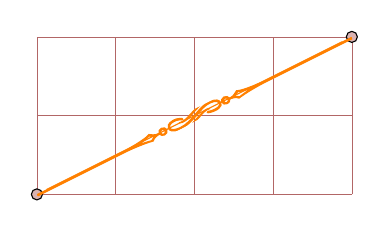
\begin{tikzpicture}
\node (A) at (0,0) {};
\node (B) at (4,2) {};
\draw [help lines,color=Maroon!60]  (0,0) grid (4,2);
\draw [fill=Maroon!30]  (A) circle (2pt) (B) circle (2pt);
\draw [orange] (A)  to [ornament=88]   (B);
\end{tikzpicture}
\end{tkzexample}

\begin{marginfigure}[-3cm]
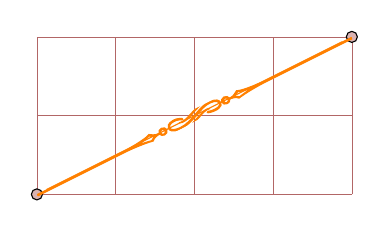
\begin{tikzpicture}
\node (A) at (0,0) {};
\node (B) at (4,2) {};
\draw [help lines,color=Maroon!60]  (0,0) grid (4,2);
\draw [fill=Maroon!30]  (A) circle (2pt) (B) circle (2pt);
\draw [orange] (A)  to [ornament=88]   (B);
\end{tikzpicture}
\caption{两节点之间的一个装饰纹样}
\end{marginfigure}

\medskip
下面的代码演示如何在两个节点之间放置两个装饰纹样。

\begin{tkzexample}[code only,very small]
  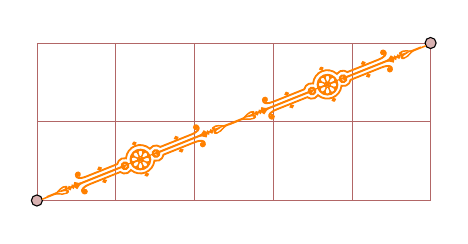
\begin{tikzpicture}
  \node (A) at (0,0) {};
  \node (B) at (5,2) {};
  \draw [help lines,color=Maroon!60]  (0,0) grid (5,2);
  \draw [fill=Maroon!30]  (A) circle (2pt) (B) circle (2pt);
  \path (A)--(B) coordinate[pos=.5] (c1);
  \draw [orange] (A)  to [ornament=84]
                 (c1) to [ornament=84] (B);
  \end{tikzpicture}
\end{tkzexample}


\begin{marginfigure}[-3cm]
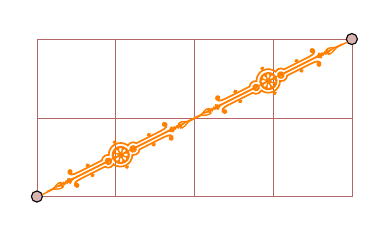
\begin{tikzpicture}
\node (A) at (0,0) {};
\node (B) at (4,2) {};
\draw [help lines,color=Maroon!60]  (0,0) grid (4,2);
\draw [fill=Maroon!30]  (A) circle (2pt) (B) circle (2pt);
\path (A)--(B) coordinate[pos=.5] (c1);
\draw [orange] (A)  to [ornament=84]
               (c1) to [ornament=84] (B);
\end{tikzpicture}
\caption{两节点之间的两个装饰纹样}
\end{marginfigure}

\medskip
正五边形的示例

\begin{tkzexample}[code only,very small]
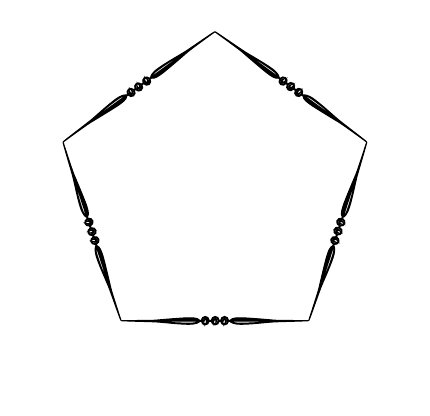
\begin{tikzpicture}[every node={anchor=center,
                                 inner sep=0pt}]
 \node[regular polygon, regular polygon sides=5,
 rotate=36,minimum size=5cm,inner sep=0pt](s)  {};
 \path (s.side 1) to [ornament=83] (s.side 2)
                  to [ornament=83] (s.side 3)
                  to [ornament=83] (s.side 4)
                  to [ornament=83] (s.side 5)
                  to [ornament=83] (s.side 1);
\end{tikzpicture}
\end{tkzexample}

\begin{marginfigure}
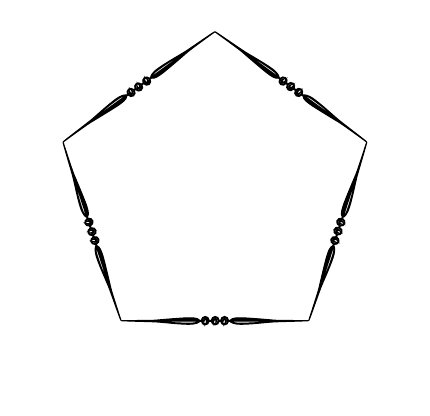
\begin{tikzpicture}[every node={anchor=center,
                                 inner sep=0pt}]
 \node[regular polygon, regular polygon sides=5,
 rotate=36,minimum size=5cm,inner sep=0pt](s)  {};
 \path (s.side 1) to [ornament=83] (s.side 2)
                  to [ornament=83] (s.side 3)
                  to [ornament=83] (s.side 4)
                  to [ornament=83] (s.side 5)
                  to [ornament=83] (s.side 1);
\end{tikzpicture}
\caption{一个正五边形}
\end{marginfigure}

\subsection{如何使用 \tkzname{ornament/at} 选项} \index{ornament/at}
\label{sub:how_to_use_the_option_at}

可以将装饰纹样沿线段 AB 移动。只需写出 \tkzname{at = number}，其中 number 是百分比，用法与 \tkzname{pos} 类似。
\begin{tkzexample}[code only,very small]
  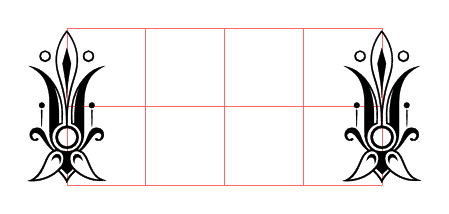
\begin{tikzpicture}
  \node (A) at (0,0) {};
  \node (B) at (4,0) {};
  \draw [help lines,color=red!60]  (0,-1) grid (4,1);
  \path  (A.center)  to [ornament=67,ornament/at=0,
                options/.append style={scale=.25}]   (B.center);
  \path  (A.center)  to [ornament=67,ornament/at=1,
                options/.append style={scale=.25}]   (B.center);
  \end{tikzpicture}
\end{tkzexample}

\begin{marginfigure}
  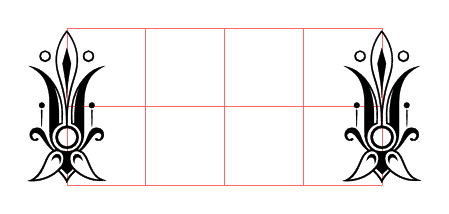
\begin{tikzpicture}
  \node (A) at (0,0) {};
  \node (B) at (4,0) {};
  \draw [help lines,color=red!60]  (0,-1) grid (4,1);
  \path  (A.center)  to [ornament=67,ornament/at=0,
                options/.append style={scale=.25}]   (B.center);
  \path  (A.center)  to [ornament=67,ornament/at=1,
                options/.append style={scale=.25}]   (B.center);
  \end{tikzpicture}
  \caption{at 选项}
\end{marginfigure}


\subsection{如何使用 \tkzname{options} 选项}
\label{sub:how_to_use_the_option_options}

如果某个装饰纹样位置不理想，可以将其向上或向下移动。请查看代码，了解如何使用 \tkzname{options}。  \index{options}

\begin{tkzexample}[code only,very small]
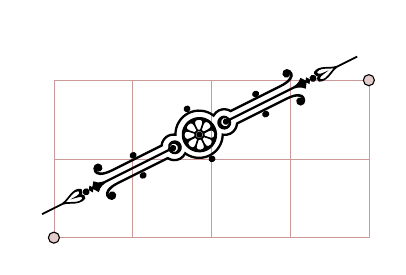
\begin{tikzpicture}
\node (A) at (0,0) {};
\node (B) at (4,2) {};
\draw [help lines,color=Maroon!40]  (0,0) grid (4,2);
\draw [fill=Maroon!20]  (A) circle (2pt) (B) circle (2pt);
\path  (A.center) to [ornament=84,
       options/.append style={yshift=10pt}] (B.center);
\end{tikzpicture}
\end{tkzexample}

\begin{marginfigure}[-3cm]
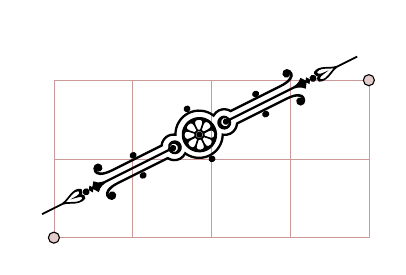
\begin{tikzpicture}
\node (A) at (0,0) {};
\node (B) at (4,2) {};
\draw [help lines,color=Maroon!40]  (0,0) grid (4,2);
\draw [fill=Maroon!20]  (A) circle (2pt) (B) circle (2pt);
\path  (A.center) to [ornament=84,
        options/.append style={yshift=10pt}] (B.center);
\end{tikzpicture}
\caption{options 的用法}
\end{marginfigure}

\section{如何制作一行装饰纹样}
\subsection{使用 chains 库}
\begin{marginfigure}

\begin{tikzpicture}
  \node[draw,circle,minimum size=4pt,inner sep=0] (A) at (0,0){};
  \coordinate (B) at (8,0);
  {[start chain,node distance=0,inner sep=0]
  \node[anchor=west] [on chain] at (A){\pgfornament[width=1cm]{70}};
\node [on chain] {\pgfornament[width=1cm]{70}};
\node [on chain] {\pgfornament[width=1cm]{70}};
\node [on chain] {\pgfornament[width=1cm]{70}};}
  \end{tikzpicture}
  \caption{使用 \doclib{chains} 库排列的装饰行}
\end{marginfigure}

\begin{tkzexample}[code only,very small]

\begin{tikzpicture}
\node[draw,circle,
     minimum size=4pt,inner sep=0] (A) at (0,0){};
\coordinate (B) at (8,0);
{[start chain,node distance=0,inner sep=0]
\node[anchor=west] [on chain] at (A){\pgfornament[width=1cm]{70}};
\node [on chain] {\pgfornament[width=1cm]{70}};
\node [on chain] {\pgfornament[width=1cm]{70}};
\node [on chain] {\pgfornament[width=1cm]{70}};}
\end{tikzpicture}
\end{tkzexample}

\subsection{使用宏 \doccmd{pgfornamentline}}

剖析这个宏：它需要 4 个必选参数——首先是两个点，装饰行将置于这两点之间；然后是用于构成该行的装饰纹样数量；当然还有装饰纹样的编号。
另有一个可选参数用于设置各种选项。

\begin{marginfigure}
  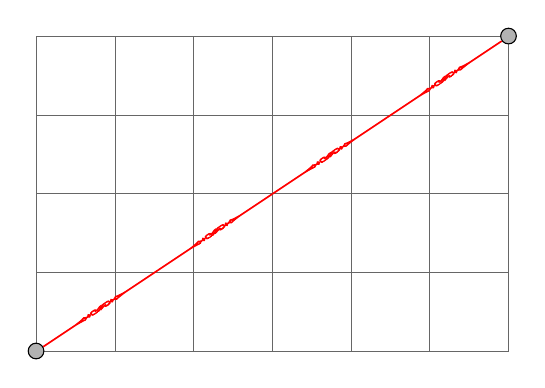
\begin{tikzpicture}[bullet/.style={circle,draw,fill=black!30,inner sep=2pt}]
  \draw [help lines,color=black!60]  (0,0) grid (6,4);
  \node[bullet] (A) at (0,0) {};
  \node[bullet] (B) at (6,4) {};
  \pgfornamentline[color=red]{A}{B}{4}{88}
  \end{tikzpicture}
  \caption{一行装饰纹样}
\end{marginfigure}

\begin{tkzexample}[code only, very small]
  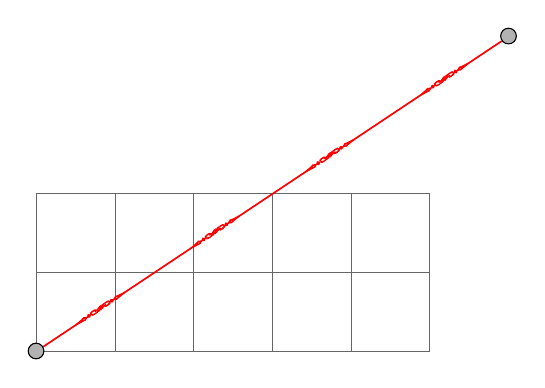
\begin{tikzpicture}[bullet/.style={%
            circle,draw,fill=black!30,inner sep=2pt}]
  \draw [help lines,color=black!60]  (0,0) grid (5,2);
  \node[bullet] (A) at (0,0) {};
  \node[bullet] (B) at (6,4) {};
  \pgfornamentline[color=red]{A}{B}{4}{88}
  \end{tikzpicture}
\end{tkzexample}



\section{使用 \doclib{chains} 在圆周上排列装饰纹样}
\begin{marginfigure}
  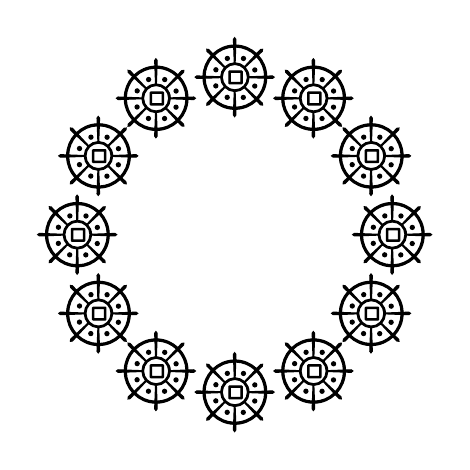
\begin{tikzpicture}[start chain=circle placed {at=(\tikzchaincount*30:2)}]
  \foreach \i in {1,...,12} \node [on chain] {\pgfornament[width=1cm]{4}};
  \end{tikzpicture}
  \caption{一个布满装饰纹样的圆}
\end{marginfigure}

\begin{tkzexample}[code only,very small]
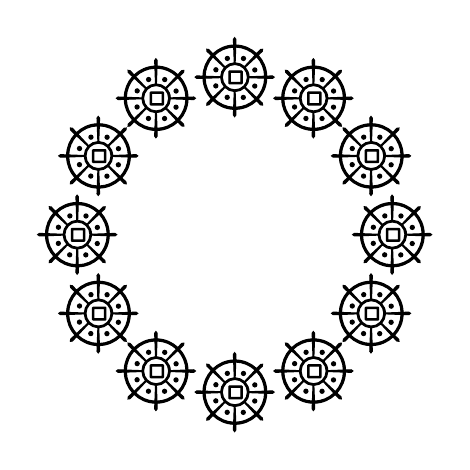
\begin{tikzpicture}[start chain=circle placed %
     {at=(\tikzchaincount*30:2)}]
\foreach \i in {1,...,12} \node [on chain]%
    {\pgfornament[width=1cm]{4}};
\end{tikzpicture}
\end{tkzexample}


\section{Vectorian 纹样库}
\label{sec:vectorian}
\subsection{装饰纹样：Vectorian 符号}
\label{sec:ornaments_symbols}
以下列出前三十个纹样元素。
\subsection{符号（第一部分）}
\label{sub:symbol1}
\index{ornament!symbols1a}
\ornamentview{1,...,30,97,98,140,141}%
\label{tab:ornaments : symbol1}

\subsection{符号（第二部分）}
\label{sub:symbol2}
接下来这一组是装饰符号，设计更为精巧。请注意索引范围从六十五到七十九。
\index{ornament!symbols2}%
\parindent=0pt

\medskip
\ornamentview{65,...,79}%
\label{tab:ornaments : symbol2}

\subsection{装饰纹样：Vectorian 角饰}
\label{sec:corners}
接下来这一组纹样用于放置在图形的四个角落。其中一半并不需要单独使用，因为它们可以由另一半通过对称得到。

\index{ornament!corners1}
\ornamentview{31,...,42,61,62,63,64}%
\label{tab:ornaments : corners1}

\index{ornament!corners2}
\ornamentview{131,132,194,195}%
\label{tab:ornaments : corners2}

\subsection{装饰纹样：Vectorian 线条}
\label{sec:lines}
接下来这一组是用于构成线条的符号。
\index{ornament!lines}

\medskip
\ornamentview{80,89}%
\label{tab:ornaments : lines}

\subsection{装饰纹样：动物}
\label{sec:animal }
接下来这一组是以动物为主题的符号。
\index{ornament!Animals}

\medskip
\ornamentview{90,91,100,102,104,106,107,108,109,110,111,112,113,122,123,124,158,159,133,134,135,136,156,157,158,159,190,193,137}%
\label{tab:ornaments : animal}

\subsection{装饰纹样：手}
\label{sec:hands }
注意：纹样 154 与 155 相同，只是尺寸更小。

\medskip
\ornamentview{152,153,154,155}%
\label{tab:ornaments : hands}

\subsection{装饰纹样：人物}
\label{sec:humans}
注意：纹样 143 与 144、145 与 146 分别相同，只是尺寸不同。

\medskip
\ornamentview{95,103,105,125,143,144,160,164}%
\label{tab:ornaments : humans}

\subsection{装饰纹样：物品}
\label{tab:ornaments : objects}

\medskip
\ornamentview{92,...,95,114,...,121,126,...,131,147,148,151,162,...,189,191,192}

\newpage
\section{中国传统纹样}

这套中国纹样库是两个人的合作成果：\emph{LianTze Lim} 与 \emph{Chennan Zhang}。他们尝试借助 \texttt{pgfornament} 已有的机制来提供一些汉族风格的传统图案。所有图案最终由 \emph{Chennan Zhang} 在 CAD 中定稿，用 TikZ 绘制，再由 \emph{LianTze Lim} 转换为适配 \texttt{pgfornament} 机制的宏包代码。这个宏包名为 \texttt{pgfornament-han}。现在我已将这些图案直接整合进来……
\ClearShipoutPictureBG
\newpgfornamentfamily{pgfhan}

\begingroup
\color{MidnightBlue}
\subsection{用于连接单线的角饰符号}
\label{sub:corner simple}
\ornamentview{1,...,8}%

\subsection{用于连接双线的角饰符号}
\label{sub:corner double}
\ornamentview{9,...,14}%

\subsection{角饰符号}
\label{sub:corner symbols}
\ornamentview{19,...,28}%

\subsection{单线、双线、直线}
\label{sub:corner symbols}
\ornamentview{29,...,32}%

\subsection{其他符号}
\label{sub:other symbols}
\ornamentview{33,...,78}%
\endgroup


\newpgfornamentfamily{vectorian}


\subsection{页面四周的边框}
以下是为页面添加边框的代码：
\begin{tkzexample}[code only,very small]
\AddToShipoutPicture{%
\begingroup
\setlength{\@tempdima}{2mm}%
\setlength{\@tempdimb}{\paperwidth-\@tempdima-1cm}%
\setlength{\@tempdimc}{\paperheight-\@tempdima}%
\put(\LenToUnit{\@tempdima},\LenToUnit{\@tempdimc}){%
  \pgfornament[color=Maroon,anchor=north west,width=1cm]{39}}
\put(\LenToUnit{\@tempdima},\LenToUnit{\@tempdima}){%
  \pgfornament[color=Maroon,anchor=south west,width=1cm,symmetry=h]{39}}
\put(\LenToUnit{\@tempdimb},\LenToUnit{\@tempdimc}){%
  \pgfornament[color=Maroon,anchor=north east,width=1cm,symmetry=v]{39}}
\put(\LenToUnit{\@tempdimb},\LenToUnit{\@tempdima}){%
  \pgfornament[color=Maroon,anchor=south east,width=1cm,symmetry=c]{39}}
\endgroup
}
\let\strippt\strip@pt
\end{tkzexample}

\clearpage\newpage
\newpage
\section{凯尔特结}
\label{sec:celtic}
\docfamily{celtic} 族包含十六个凯尔特结纹样。它们取自
\url{https://publicdomainvectors.org} 的 \emph{Ornaments vector pack}，
该素材以公有领域（\emph{“你可以复制、修改、再分发并将该图片用于任意商业用途，无需征得许可”}）
发布。这些图形通过脚本 \texttt{svg2pgf.py}（位于 \texttt{tools} 文件夹）转换，
该脚本读取 \texttt{svg}、\texttt{eps} 或 \texttt{pdf} 文件，并生成 \texttt{.pgf} 文件
以及纹样库 \texttt{pgfornament-lib-celtic.code.tex}。

\begin{tkzexample}[code only,very small]
  \usepackage[object=celtic]{pgfornament}
  ...
  \pgfornament[width=2cm,color=Maroon]{9}
\end{tkzexample}

\newpgfornamentfamily{celtic}
\begingroup
\color{MidnightBlue}
\ornamentview{1,...,16}%
\endgroup
\newpgfornamentfamily{vectorian}

\section{应用：在角落放置装饰}
\label{sec:application_placement}
注意：角饰的宽高相同（宽 = 高）。

\begin{figure}[h!]
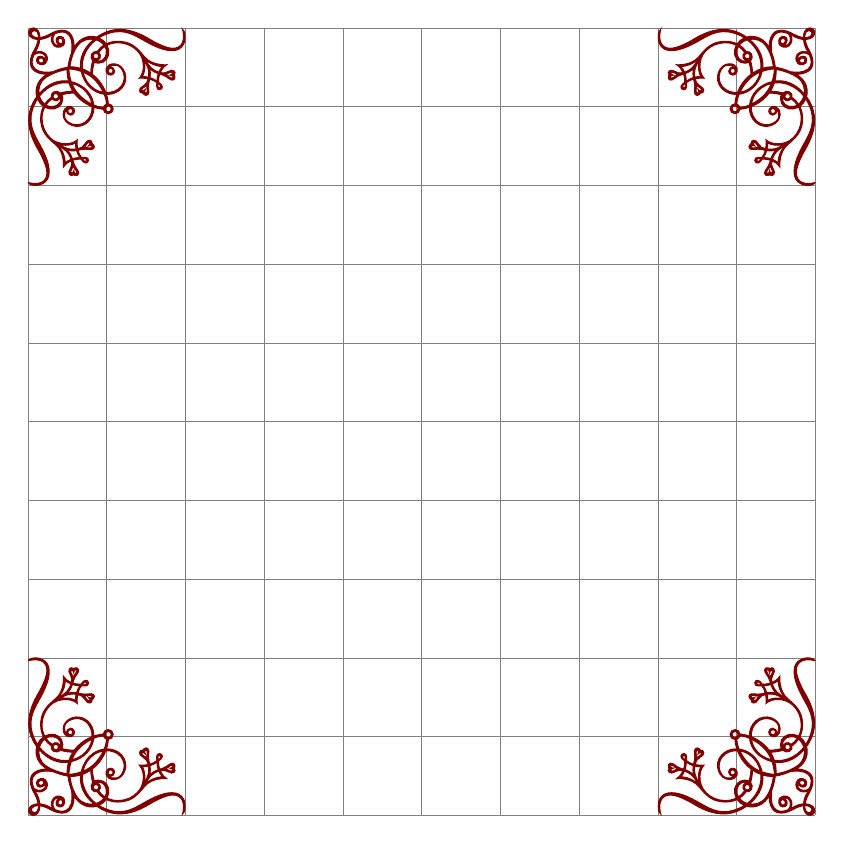
\begin{tikzpicture}[color=Maroon,every node/.style={inner sep=0pt}]
\draw[help lines] (-5,-5) grid (5,5);
\node[minimum size=10cm](vecbox){};
\node[anchor=north west] at (vecbox.north west){\pgfornament[width=2cm]{61}};
\node[anchor=north east] at (vecbox.north east){\pgfornament[width=2cm,symmetry=v]{61}};
\node[anchor=south west] at (vecbox.south west){\pgfornament[width=2cm,symmetry=h]{61}};
\node[anchor=south east] at (vecbox.south east){\pgfornament[width=2cm,symmetry=c]{61}};
\end{tikzpicture}
\caption{在角落放置装饰}
\end{figure}


\begin{tkzexample}[code only,very small]
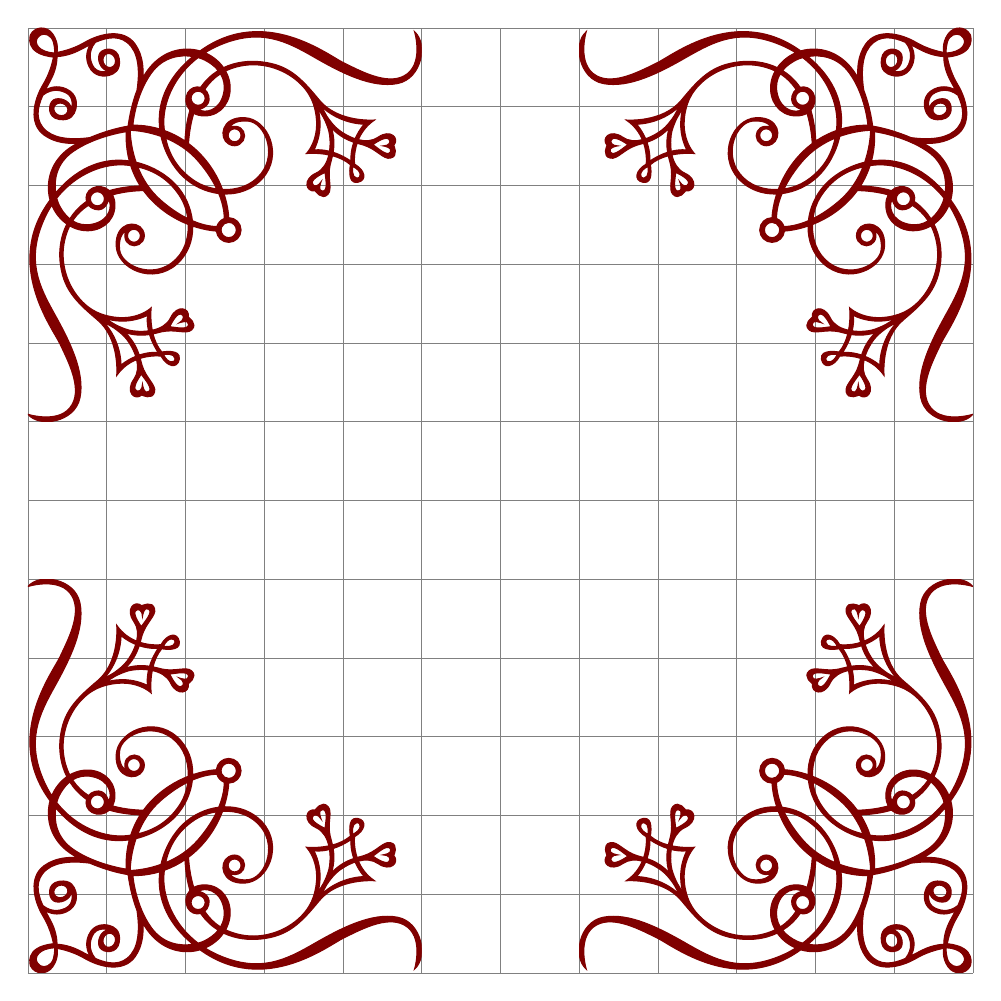
\begin{tikzpicture}[color=Maroon,
                    every node/.style={inner sep=0pt}]
 \draw[help lines] (-6,-6) grid (6,6);
 \node[minimum size=12cm](vecbox){};
 \node[anchor=north west] at (vecbox.north west)
      {\pgfornament[width=5cm]{61}};
 \node[anchor=north east] at (vecbox.north east)
      {\pgfornament[width=5cm,symmetry=v]{61}};
 \node[anchor=south west] at (vecbox.south west)
      {\pgfornament[width=5cm,symmetry=h]{61}};
 \node[anchor=south east] at (vecbox.south east)
      {\pgfornament[width=5cm,symmetry=c]{61}};
\end{tikzpicture}
\end{tkzexample}
\index{minimum size}
\index{anchor}

\section{应用：为页面创建边框}

\begin{tikzpicture}[remember picture, overlay]
\node[anchor=north west] (nw) at (current page.north west){%
\pgfornament[width=2cm]{63}};
\node[anchor=north east] (ne) at (current page.north east){%
\pgfornament[width=2cm,symmetry=v]{63}};
\node[anchor=south west] (sw) at (current page.south west){%
\pgfornament[width=2cm,symmetry=h]{63}};
\node[anchor=south east] (se) at (current page.south east){%
\pgfornament[width=2cm,symmetry=c]{63}};
\coordinate (nw) at ([shift={(-.82cm,-1cm)}]nw);
\coordinate (sw) at ([shift={(-.82cm,+1cm)}]sw);
\coordinate (ne) at ([shift={(+.82cm,-1cm)}]ne);
\coordinate (se) at ([shift={(+.82cm,+1cm)}]se);
\pgfornamentline[color=Maroon]{nw}{sw}{4}{88}
\pgfornamentline[color=Maroon]{ne}{se}{4}{88}
\coordinate (nw) at ([shift={(1.8 cm,1.845 cm)}]nw);
\coordinate (ne) at ([shift={(-1.8 cm,1.845 cm)}]ne);
\pgfornamentline[color=Maroon]{nw}{ne}{3}{88}
\coordinate (sw) at ([shift={(1.8 cm,-1.845 cm)}]sw);
\coordinate (se) at ([shift={(-1.8 cm,-1.845 cm)}]se);
\pgfornamentline[color=Maroon]{sw}{se}{3}{88}
\pgfornamentline[color=Maroon]{sw}{se}{3}{88}
\end{tikzpicture}


\section{应用：文本周围的装饰框}
\label{sec:application_poem}
我选了一首诗来演示这个主题。


\begin{center}
\begin{figure}[h!]
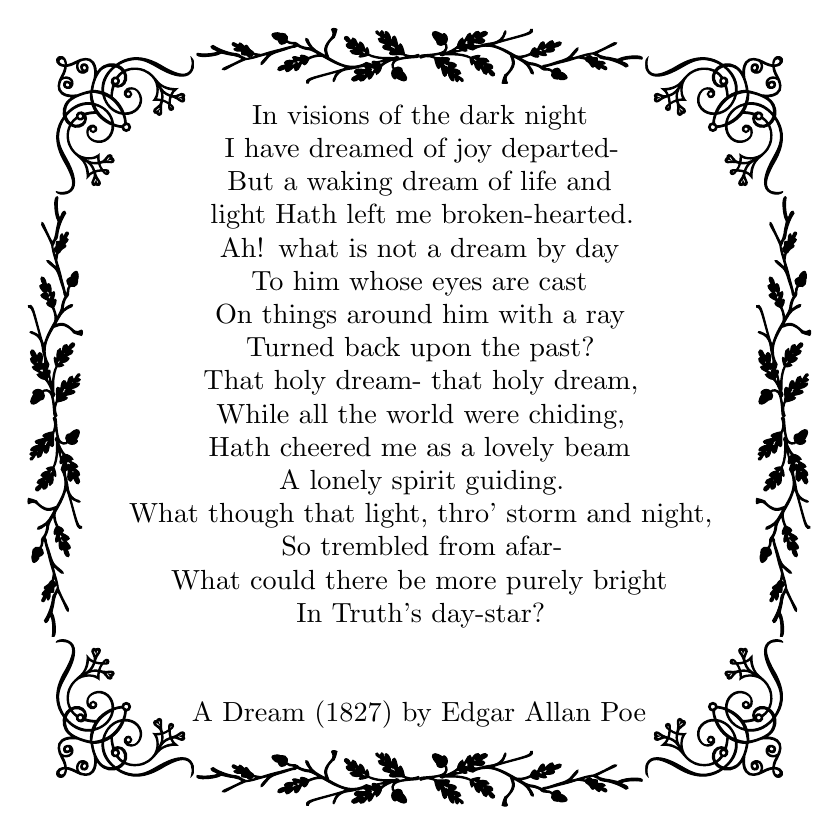
\begin{tikzpicture}
  \node[text width=8cm,align=center](Text){%
  In visions of the dark night\\
  I have dreamed of joy departed-\\
  But a waking dream of life and light\
  Hath left me broken-hearted.\\

  Ah! what is not a dream by day\\
  To him whose eyes are cast \\
  On things around him with a ray \\
  Turned back upon the past? \\

  That holy dream- that holy dream,\\
  While all the world were chiding,\\
  Hath cheered me as a lovely beam\\
  A lonely spirit guiding.\\

  What though that light, thro' storm and night,\\
  So trembled from afar- \\
  What could there be more purely bright \\
  In Truth's day-star? \\
  \vspace{24pt}
   A Dream (1827) by Edgar Allan Poe
  } ;

\node[inner sep=0pt,shift={(-.5cm,.5cm)},anchor=north west](CNW)  at (Text.north west)
    {\pgfornament[width=1.75cm]{61}};
\node[inner sep=0pt,shift={(.5cm,.5cm)},anchor=north east](CNE)   at (Text.north east)
    {\pgfornament[width=1.75cm,symmetry=v]{61}};
\node[inner sep=0pt,shift={(-.5cm,-.5cm)},anchor=south west](CSW) at (Text.south west)
     {\pgfornament[width=1.75cm,symmetry=h]{61}};
\node[inner sep=0pt,shift={(.5cm,-.5cm)},anchor=south east](CSE)  at (Text.south east)
     {\pgfornament[width=1.75cm,symmetry=c]{61}};
 \pgfornamenthline{CNW}{CNE}{north}{87}
\pgfornamenthline{CSW}{CSE}{south}{87}
\pgfornamentvline{CNW}{CSW}{west}{87}
\pgfornamentvline{CNE}{CSE}{east}{87}
\end{tikzpicture}
\caption{一首诗}
\end{figure}
\end{center}

这首诗被放在一个名为 \Verb+Text+ 的节点中。
然后我们可以相对于节点 \Verb+Text+ 的四个锚点来放置四个角饰。
最后，借助宏 \doccmd{pgfornamenthline} 和 \doccmd{pgfornamentvline}，即可完成整个边框。

\begin{tkzexample}[code only,very small]

\begin{tikzpicture}[every node/.style={inner sep=0pt}]
\node[text width=8cm,align=center](Text){%
    In visions of the dark night ...} ;
\node[shift={(-1cm,1cm)},anchor=north west](CNW)
at (Text.north west) {\pgfornament[width=1.75cm]{61}};
\node[shift={(1cm,1cm)},anchor=north east](CNE)
at (Text.north east) {\pgfornament[width=1.75cm,symmetry=v]{61}};
\node[shift={(-1cm,-1cm)},anchor=south west](CSW)
at (Text.south west) {\pgfornament[width=1.75cm,symmetry=h]{61}};
\node[shift={(1cm,-1cm)},anchor=south east](CSE)
at (Text.south east) {\pgfornament[width=1.75cm,symmetry=c]{61}};
\pgfornamenthline{CNW}{CNE}{north}{87}
\pgfornamenthline{CSW}{CSE}{south}{87}
\pgfornamentvline{CNW}{CSW}{west}{87}
\pgfornamentvline{CNE}{CSE}{east}{87}
\end{tikzpicture}
\end{tkzexample}

\section{应用：框内文本}
\label{sec:frame}
首先借助节点搭出边框，然后再把文本作为一个节点相对于其他节点放置。

\begin{figure}[h!]
\begin{center}
\newcommand{\framesize}{8 cm}
\begin{tikzpicture}[color=Maroon,
                   transform shape,
                   every node/.style={inner sep=0pt}]
\node[minimum size=\framesize,fill=Beige!20](vecbox){};
\node[anchor=north west] at (vecbox.north west){%
      \pgfornament[width=0.2*\framesize]{63}};
\node[anchor=north east] at (vecbox.north east){%
                         \pgfornament[width=0.2*\framesize,symmetry=v]{63}};
\node[anchor=south west] at (vecbox.south west){%
      \pgfornament[width=0.2*\framesize,symmetry=h]{63}};
\node[anchor=south east] at (vecbox.south east){%
      \pgfornament[width=0.2*\framesize,symmetry=c]{63}};
\node[anchor=north] at (vecbox.north){%
      \pgfornament[width=0.6*\framesize,symmetry=h]{46}};
\node[anchor=south] at (vecbox.south){%
      \pgfornament[width=0.6*\framesize]{46}};
\node[anchor=north,rotate=90]  at (vecbox.west){%
      \pgfornament[width=0.6*\framesize,symmetry=h]{46}};
\node[anchor=north,rotate=-90] at (vecbox.east){%
      \pgfornament[width=0.6*\framesize,symmetry=h]{46}};
\node[inner sep=6pt] (text) at (vecbox.center){\Huge Ornaments};
\node[anchor=north] at (text.south){%
      \pgfornament[width=0.5*\framesize]{75}};
\node[anchor=south] at (text.north){%
      \pgfornament[width=0.5*\framesize,symmetry=h]{75}};
\end{tikzpicture}
\caption{在 tikzpicture 环境中实现的框内文本}
\end{center}
\end{figure}

\begin{tkzexample}[code only,very small]
\newcommand{\framesize}{8 cm}
\begin{tikzpicture}[color=Maroon,
                   transform shape,
                   every node/.style={inner sep=0pt}]
\node[minimum size=\framesize,fill=Beige!10](vecbox){};
\node[anchor=north west] at (vecbox.north west){%
      \pgfornament[width=0.2*\framesize]{63}};
\node[anchor=north east] at (vecbox.north east){%
      \pgfornament[width=0.2*\framesize,symmetry=v]{63}};
\node[anchor=south west] at (vecbox.south west){%
      \pgfornament[width=0.2*\framesize,symmetry=h]{63}};
\node[anchor=south east] at (vecbox.south east){%
      \pgfornament[width=0.2*\framesize,symmetry=c]{63}};
\node[anchor=north] at (vecbox.north){%
      \pgfornament[width=0.6*\framesize,symmetry=h]{46}};
\node[anchor=south] at (vecbox.south){%
      \pgfornament[width=0.6*\framesize]{46}};
\node[anchor=north,rotate=90]  at (vecbox.west){%
      \pgfornament[width=0.6*\framesize,symmetry=h]{46}};
\node[anchor=north,rotate=-90] at (vecbox.east){%
      \pgfornament[width=0.6*\framesize,symmetry=h]{46}};
\node[inner sep=6pt] (text) at (vecbox.center){\Huge Ornaments};
\node[anchor=north] at (text.south){%
      \pgfornament[width=0.5*\framesize]{75}};
\node[anchor=south] at (text.north){%
      \pgfornament[width=0.5*\framesize,symmetry=h]{75}};
\end{tikzpicture}
\end{tkzexample}
\index{transform shape}
\index{color}
\index{every node}

\section{应用：绘制五边形的另一种方法}
\label{sec:application_other_way_to_get_a_pentagon}
我们既可以手动放置纹样，也可以使用上一种方法。
\sidenote{\tkzcname{getornamentlength} 的作用是……}

\begin{tkzexample}[code only,very small]
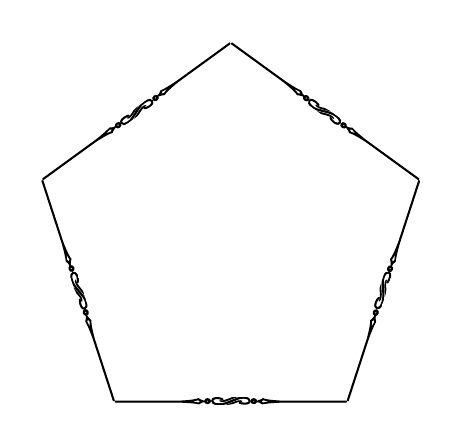
\begin{tikzpicture}[every node={anchor=center,inner sep=0pt}]
    \node[regular polygon,
          regular polygon sides=5,
          minimum size=5cm,
          inner sep=0pt](s)  {};
    \getornamentlength{s}{corner 1}{s}{corner 2}
    \node[rotate=216] at (s.side 1)
         {\pgfornament[width=\ornamentlen]{88}};
    \node[rotate=288] at (s.side 2)
         {\pgfornament[width=\ornamentlen]{88}};
    \node[rotate=0]   at (s.side 3)
         {\pgfornament[width=\ornamentlen]{88}};
    \node[rotate=72]  at (s.side 4)
         {\pgfornament[width=\ornamentlen]{88}};
    \node[rotate=144] at (s.side 5)
         {\pgfornament[width=\ornamentlen]{88}};
\end{tikzpicture}
\end{tkzexample}  \index{rotate}   \index{regular polygon}


\begin{marginfigure}[-1cm]
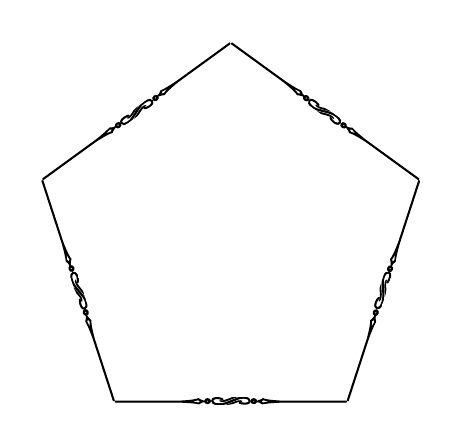
\begin{tikzpicture}[every node={anchor=center,inner sep=0pt}]
\node[regular polygon, regular polygon sides=5,
      minimum size=5cm,inner sep=0pt](s)  {};
\getornamentlength{s}{corner 1}{s}{corner 2}
\node[rotate=216] at (s.side 1){\pgfornament[width=\ornamentlen]{88}};
\node[rotate=288] at (s.side 2){\pgfornament[width=\ornamentlen]{88}};
\node[rotate=0]   at (s.side 3){\pgfornament[width=\ornamentlen]{88}};
\node[rotate=72]  at (s.side 4){\pgfornament[width=\ornamentlen]{88}};
\node[rotate=144] at (s.side 5){\pgfornament[width=\ornamentlen]{88}};
\end{tikzpicture}
\caption{一个五边形}
\end{marginfigure}

\vspace{60pt}

\section{\docpkg{tikzrput} 宏包}
\label{sec:package_rput}

Pstricks 用户习惯于使用 \doccmd{rput}\index{rput} 来放置对象，因此我创建了一个仅含单个宏 \tkzcname{rput} 的 \tkzname{\docpkg{tikzrput}} 宏包。该宏的用法与 Pstricks 中的同名宏完全一致，参数和选项也相同。除你正在阅读的本文档之外，你还可以找到关于该宏包的独立文档。将对象显示在点 $(x,y)$ 处，是借助 \emph{pstricks} 的 \verb|\rput| 来实现的，用法如下：\par\medskip

\begin{docspec}
 \color{black} \doccmd{rput}[\docopt{refpoint}]\{\docarg{angle}\}%
\docparen{x,y}\{\doccmd{pgfornament[\docopt{options}]\{\docarg{number}\}}\}
\end{docspec}

\subsection{使用 \tkzcname{rput} 的示例}
\label{sub:example_with_rput}

\begin{tkzexample}[code only,very small]
\foreach \a in {0,4,...,356}{%
  \rput(\a;2){$\bullet$}%
  }
    \rput[B](0;0){Circle}%
\end{tkzexample}  \Imacro{foreach}

\begin{marginfigure}[-3cm]
\hspace*{2cm}
  \foreach \a in {0,16,...,356}{%
    \rput(\a;2){$\bullet$}%
    }
      \rput[B](0;0){Circle}%

  \vspace*{3cm}
      \caption{使用 \tkzcname{rput} 的示例}
\end{marginfigure}

\subsection{配合 \tkzcname{rput} 使用装饰纹样}
\label{sub:ornament_with}

\setlength{\fboxsep}{0pt}

\begin{tkzexample}[code only,very small]
\begin{picture}(5,4)
 \rput(2,1){\pgfornament[width=2cm]{1}}
 \rput(4,2){\pgfornament[width=2cm]{2}}
\end{picture}
\end{tkzexample} \Imacro{rput}

\begin{marginfigure}
  \begin{picture}(5,4)
   \rput(2,1){\pgfornament[color=CadetBlue,width=2cm]{1}}
   \rput(4,2){\pgfornament[color=CadetBlue,width=2cm]{2}}
  \end{picture}
 \caption{使用 rput 放置装饰纹样}
\end{marginfigure}

\section{来自 pgfornamenthan 的示例}
\label{sec:pgfornamenthan}
\ClearShipoutPictureBG
\newpgfornamentfamily{pgfhan}

\subsection{LianTze Lim 示例 1}
\label{sub:LianTze1}
\url{https://github.com/liantze/pgfornament-han}

\begin{marginfigure}
\begin{center}

\begin{tikzpicture}
\tikzset{every node/.append style={inner sep=0pt,color=MidnightBlue!50}}
\tikzset{pgfornamentstyle/.style={draw=green!20!black,
           fill=orange,fill opacity=.5,thick}}%
\node (nw) {\pgfornament[scale=0.25]{12}};
\node[right=50bp of nw] (ne) {\pgfornament[scale=0.25,symmetry=v]{12}};
\node[below=50bp of nw] (sw) {\pgfornament[scale=0.25,symmetry=h]{12}};
\node[below=50bp of ne] (se) {\pgfornament[scale=0.25,symmetry=c]{12}};
\node[anchor=north west] at (nw.north east) {\pgfornament[scale=0.25]{32}};
\node[anchor=south west] at (sw.south east) {\pgfornament[scale=0.25]{32}};
\node[anchor=south west,rotate=-90] at (nw.south west)
                                  {\pgfornament[scale=0.25]{32}};
\node[anchor=south east,rotate=90] at (ne.south east)
                                  {\pgfornament[scale=0.25]{32}};

\node[anchor=center,shift={(25bp,-25bp)}] at (nw.south east) {\pgfornament[scale=0.5]{57}};
\end{tikzpicture}
\caption{LianTze Lim 示例 1}
\end{center}
\end{marginfigure}
\begin{tkzexample}[code only,very small]

\begin{tikzpicture}
\tikzset{every node/.append style={inner sep=0pt,color=MidnightBlue!50}}
\tikzset{pgfornamentstyle/.style={draw=green!20!black,
           fill=orange,fill opacity=.5,thick}}%
\node (nw) {\pgfornament[scale=0.25]{12}};
\node[right=50bp of nw] (ne){\pgfornament[scale=0.25,symmetry=v]{12}};
\node[below=50bp of nw] (sw){\pgfornament[scale=0.25,symmetry=h]{12}};
\node[below=50bp of ne] (se){\pgfornament[scale=0.25,symmetry=c]{12}};
\node[anchor=north west] at (nw.north east)%
             {\pgfornament[scale=0.25]{32}};
\node[anchor=south west] at (sw.south east)%
             {\pgfornament[scale=0.25]{32}};
\node[anchor=south west,rotate=-90] at (nw.south west)
                            {\pgfornament[scale=0.25]{32}};
\node[anchor=south east,rotate=90] at (ne.south east)
                            {\pgfornament[scale=0.25]{32}};
\node[anchor=center,shift={(25bp,-25bp)}] at (nw.south east)
 {\pgfornament[scale=0.5]{57}};
\end{tikzpicture}
\end{tkzexample}

\subsection{LianTze Lim 示例 2}


\begin{marginfigure}
\begin{center}

\begin{tikzpicture}
\tikzset{every node/.append style={color=Goldenrod,inner sep=0pt}}
\node (nw) {\pgfornament[scale=0.25]{23}};
\node[right=53bp of nw] (ne)
     {\pgfornament[scale=0.25,symmetry=v]{23}};
\node[anchor=north west,xshift=-2bp] at (nw.north east)
     {\pgfornament[scale=0.25]{41}};
\node[anchor=north east,xshift=2bp] at (ne.north west)
     {\pgfornament[scale=0.25,symmetry=v]{41}};
\end{tikzpicture}
\end{center}
\caption{LianTze Lim 示例 2}
\end{marginfigure}
\begin{tkzexample}[code only,very small]

\begin{tikzpicture}
\tikzset{every node/.append style={color=Goldenrod,inner sep=0pt}}
\node (nw) {\pgfornament[scale=0.25]{23}};
\node[right=53bp of nw] (ne){\pgfornament[scale=0.4,symmetry=v]{23}};
 \node[anchor=north west,xshift=8bp] at (nw.north east)
  {\pgfornament[scale=0.25]{41}};
\node[anchor=north east,xshift=-8bp] at (ne.north west)
  {\pgfornament[scale=0.25,symmetry=v]{41}};
\end{tikzpicture}
\end{tkzexample}


\clearpage\newpage
\subsection{示例 3（基于 LianTze Lim 的一个示例）}
\newpgfornamentfamily{pgfhan}

\newbox{\fortyseven}
\savebox{\fortyseven}{\pgfornament[scale=0.20,color=MidnightBlue]{47}}
\tikzset{every node/.append style={inner sep=0pt}}
\AddToShipoutPictureBG{\begin{tikzpicture}[overlay,remember picture,color=MidnightBlue]
\node[anchor=north west,shift={(0.7,-0.85)}] at (current page.north west)
  (nw) {\pgfornament[scale=0.2]{25}};
\node[anchor=north east,shift={(-0.7,-0.85)}] at (current page.north east)
  (ne) {\pgfornament[scale=0.2,symmetry=v]{25}};
\node[anchor=south west,shift={(0.7,0.85)}] at (current page.south west)
  (sw) {\pgfornament[scale=0.2,symmetry=h]{25}};
\node[anchor=south east,shift={(-0.7,0.85)}] at (current page.south east)
  (se) {\pgfornament[scale=0.2,symmetry=c]{25}};
\begin{scope}[start chain,node distance=-3pt]
\node[anchor=north west,on chain] at (nw.north east) {\usebox{\fortyseven}};
\foreach \i in {1,...,14} {\node[on chain]{\usebox{\fortyseven}};}
\end{scope}
 \begin{scope}[start chain,node distance=-3pt]
 \node[anchor=south west,on chain] at (sw.south east) {\usebox{\fortyseven}};
 \foreach \i in {1,...,6} \node[on chain]{\usebox{\fortyseven}};
 \end{scope}
\begin{scope}[start chain=going left,node distance=-3pt]
\node[anchor=south east,on chain,xshift={3pt}] at (se.south west) {\usebox{\fortyseven}};
\foreach \i in {1,...,6} \node[on chain]{\usebox{\fortyseven}};
\end{scope}
\foreach \i in {0,...,22}
  \node[anchor=south west,rotate=-90,shift={($\i*(31bp,0)$)}] at (nw.south west)
    {\usebox{\fortyseven}};
\foreach \i in {0,...,22}
  \node[anchor=south east,rotate=90,shift={($\i*(-31bp,0)$)}] at ([yshift={+3pt}]ne.south east)
    {\usebox{\fortyseven}};
\node[yshift=32pt] at (current page.south) {\pgfornament[scale=0.1]{51}};
\node[yshift=32pt,text=black] at (current page.south) {\large\thepage};
\end{tikzpicture}}

\begin{center}
\begin{tikzpicture}
  \tikzset{every node/.append style={MidnightBlue,inner sep=0pt,node distance=0pt}}
  \node (nw) {\pgfornament[scale=0.2]{6}};
  \node[right=100bp of nw] (ne){\pgfornament[scale=0.2,symmetry=v]{16}};
  \node[below=-8bp of nw] (sw) {\pgfornament[scale=0.2,symmetry=h]{16}};
  \node[below=-8bp of ne] (se) {\pgfornament[scale=0.2,symmetry=c]{6}};
  \node[anchor=north west,xscale=2.5] at (nw.north east)
       {\pgfornament[scale=0.2]{30}};
  \node[anchor=south west,xscale=2.5] at (sw.south east)
       {\pgfornament[scale=0.2]{30}};
  \node[font=\Large,text=black,shift={(50bp,4bp)}] at (nw.south east) {边框所用代码};
\end{tikzpicture}
\end{center}

\begin{tkzexample}[code only, very small]
\newpgfornamentfamily{pgfhan}
\newbox{\fortyseven}
\savebox{\fortyseven}{\pgfornament[scale=0.20,color=MidnightBlue]{47}}
\tikzset{every node/.append style={inner sep=0pt}}
\AddToShipoutPictureBG{%
\begin{tikzpicture}[overlay,remember picture,color=MidnightBlue]
\node[anchor=north west,shift={(0.7,-0.85)}] at (current page.north west)
  (nw) {\pgfornament[scale=0.2]{25}};
\node[anchor=north east,shift={(-0.7,-0.85)}] at (current page.north east)
  (ne) {\pgfornament[scale=0.2,symmetry=v]{25}};
\node[anchor=south west,shift={(0.7,0.85)}] at (current page.south west)
  (sw) {\pgfornament[scale=0.2,symmetry=h]{25}};
\node[anchor=south east,shift={(-0.7,0.85)}] at (current page.south east)
  (se) {\pgfornament[scale=0.2,symmetry=c]{25}};
\begin{scope}[start chain,node distance=-3pt]
\node[anchor=north west,on chain] at (nw.north east)
{\usebox{\fortyseven}};
\foreach \i in {1,...,14} {\node[on chain]{\usebox{\fortyseven}};}
\end{scope}
 \begin{scope}[start chain,node distance=-3pt]
 \node[anchor=south west,on chain] at (sw.south east)
 {\usebox{\fortyseven}};
 \foreach \i in {1,...,6} \node[on chain]{\usebox{\fortyseven}};
 \end{scope}
\begin{scope}[start chain=going left,node distance=-3pt]
\node[anchor=south east,on chain,xshift={3pt}] at (se.south west)
 {\usebox{\fortyseven}};
\foreach \i in {1,...,6} \node[on chain]
{\usebox{\fortyseven}};
\end{scope}
\foreach \i in {0,...,22}
\node[anchor=south west,rotate=-90,
      shift={($\i*(31bp,0)$)}] at (nw.south west)
      {\usebox{\fortyseven}};
\foreach \i in {0,...,22}
\node[anchor=south east,rotate=90,shift={($\i*(-31bp,0)$)}] at
 ([yshift={+3pt}]ne.south east){\usebox{\fortyseven}};
\node[yshift=32pt] at (current page.south){\pgfornament[scale=0.1]{51}};
\node[yshift=32pt,text=black] at (current page.south){\large\thepage};
\end{tikzpicture}
}
\end{tkzexample}

\clearpage \newpage
\subsection{示例 4（基于 LianTze Lim 的一个示例）}
\begin{figure}
\begin{newfamily}[pgfhan]
\begin{center}
  \begin{tikzpicture}
  \tikzset{every node/.append style={inner sep=0pt,color= MidnightBlue}}
  \node[minimum width=180bp,minimum height=100bp] (chframe){};
  \node[anchor=north west] (nw) at (chframe.north west)
    {\pgfornament[scale=0.25]{1}};
  \node[anchor=north east]  at (chframe.north east)
    {\pgfornament[symmetry=v,scale=0.25]{1}};
  \node[anchor=south west] (sw) at (chframe.south west)
    {\pgfornament[symmetry=h,scale=0.25]{1}};
  \node[anchor=south east]  at (chframe.south east)
    {\pgfornament[symmetry=c,scale=0.25]{1}};
   \node[anchor=south west,xscale=2] at (sw.south east)
    {\pgfornament[scale=0.25]{29}};
    \node[anchor=north west,xscale=2] at (nw.north east)
    {\pgfornament[scale=0.25]{29}};
  % circle
  \begin{scope}
  \tikzset{pgfornamentstyle/.style={draw=Goldenrod,fill=Red,line width=1pt}}
  \node[fill=MidnightBlue,circle,draw=Red,line width=2pt,inner sep=-8pt]
  at (chframe.center)  {\pgfornament[scale=0.40]{56}};
  \end{scope}
  \end{tikzpicture}
\end{center}
\end{newfamily}
\end{figure}

\begin{tkzexample}[code only, very small]
\begin{newfamily}[pgfhan]
\begin{center}
\begin{tikzpicture}
\tikzset{every node/.append style={%
        inner sep=0pt,
        color= MidnightBlue}}
\node[minimum width=180bp,minimum height=100bp] (chframe){};
\node[anchor=north west] (nw) at (chframe.north west)
  {\pgfornament[scale=0.25]{1}};
\node[anchor=north east]  at (chframe.north east)
  {\pgfornament[symmetry=v,scale=0.25]{1}};
\node[anchor=south west] (sw) at (chframe.south west)
  {\pgfornament[symmetry=h,scale=0.25]{1}};
\node[anchor=south east]  at (chframe.south east)
  {\pgfornament[symmetry=c,scale=0.25]{1}};
 \node[anchor=south west,xscale=2] at (sw.south east)
  {\pgfornament[scale=0.25]{29}};
  \node[anchor=north west,xscale=2] at (nw.north east)
  {\pgfornament[scale=0.25]{29}};
% circle
\begin{scope}
\tikzset{pgfornamentstyle/.style={draw=Goldenrod,
                                    fill=Red,
                                    line width=1pt}}
\node[fill=MidnightBlue,circle,draw=Red,
        line width=2pt,inner sep=-8pt]
  at (chframe.center) {\pgfornament[scale=0.40]{56}};
\end{scope}
\end{tikzpicture}
\end{center}
\end{newfamily}
\end{tkzexample}

\clearpage \newpage
\ClearShipoutPicture
\newpgfornamentfamily{vectorian}
\section{来自 psvectorian 的示例}
\label{sec:psvectorian}

\subsection{大标题 —— e01}
\label{sub:largetitle}
该示例可在以下地址获取：
\url{http://melusine.eu.org/syracuse/pstricks/vectorian/e01.tex}。

我借助 tikzrput 宏包中的 \Verb|rput| 宏，以相同的代码绘制出了该图。
我仅将 \doccmd{psvectorian} 替换为 \doccmd{pgfornament}。

\begin{figure}
  \begin{center}
  \rput[r](-3pt,3pt){\pgfornament[scale=.35]{72}}
  \Large{Motifs d'ornements}%
  \rput[l](3pt,3pt){\pgfornament[scale=.35]{73}}\\
  \rput(0,0){\pgfornament[scale=.5]{85}}
  \end{center}
  \caption{psvectorian 中名为 e01 的示例}
\end{figure}
\begin{tkzexample}[code only,very small]
  \rput[r](-3pt,3pt){\pgfornament[scale=.35]{72}}
  \large{Motifs d'ornements}%
  \rput[l](3pt,3pt){\pgfornament[scale=.35]{73}}\\
  \rput(0,0){\pgfornament[scale=.5]{85}}
\end{tkzexample}

\subsection{带框封面 —— e02}
该示例可在以下地址获取：

{\small\url{http://melusine.eu.org/syracuse/pstricks/vectorian/e02.tex}}

我需要使用 \docenv{tikzpicture} 和 \doccmd{draw} 来替换 \docenv{pspicture} 和 \doccmd{psframe}。

\begin{figure}
\begin{center}
  \begin{tikzpicture}[color=blue]
   \draw[use as bounding box,thin] (-5,-5) rectangle (5,5);
   \node {\rput[tl](-3,5){\pgfornament[width=6cm]{71}}
   \rput[bl](-3,-5){\pgfornament[width=6cm,,symmetry=h]{71}}
   \rput[tl](-5,5){\pgfornament[width=2cm]{63}}
   \rput[tr](5,5){\pgfornament[width=2cm,,symmetry=v]{63}}
   \rput[bl](-5,-5){\pgfornament[width=2cm,,symmetry=h]{63}}
   \rput[br](5,-5){\pgfornament[width=2cm,,symmetry=c]{63}}
   \rput[bl]{-90}(-5,3){\pgfornament[width=6cm]{46}}
   \rput[bl]{90}(5,-3){\pgfornament[width=6cm]{46}}
   \rput(0,0){\Huge Ornaments}
   \rput[t](0,-0.5){\pgfornament[width=5cm]{75}}
   \rput[b](0,0.5){\pgfornament[width=5cm]{69}}
   \rput[tr]{-30}(-1,2.5){\pgfornament[width=2cm]{57}}
   \rput[tl]{30}(1,2.5){\pgfornament[width=2cm,symmetry=v]{57}}};
   \end{tikzpicture}
\end{center}
\caption{psvectorian 中名为 e02 的示例}
\end{figure}

\begin{tkzexample}[code only,very small]
 \begin{tikzpicture}[color=blue]
  \draw[use as bounding box,thin] (-5,-5) rectangle (5,5);
  \node {\rput[tl](-3,5){\pgfornament[width=6cm]{71}}
  \rput[bl](-3,-5){\pgfornament[width=6cm,,symmetry=h]{71}}
  \rput[tl](-5,5){\pgfornament[width=2cm]{63}}
  \rput[tr](5,5){\pgfornament[width=2cm,,symmetry=v]{63}}
  \rput[bl](-5,-5){\pgfornament[width=2cm,,symmetry=h]{63}}
  \rput[br](5,-5){\pgfornament[width=2cm,,symmetry=c]{63}}
  \rput[bl]{-90}(-5,3){\pgfornament[width=6cm]{46}}
  \rput[bl]{90}(5,-3){\pgfornament[width=6cm]{46}}
  \rput(0,0){\Huge Ornaments}
  \rput[t](0,-0.5){\pgfornament[width=5cm]{75}}
  \rput[b](0,0.5){\pgfornament[width=5cm]{69}}
  \rput[tr]{-30}(-1,2.5){\pgfornament[width=2cm]{57}}
  \rput[tl]{30}(1,2.5){\pgfornament[width=2cm,symmetry=v]{57}}};
  \end{tikzpicture}
\end{tkzexample}

\vspace{30pt}
\subsection{小标题 —— e03}
该示例可在以下地址获取：

{\small\url{http://melusine.eu.org/syracuse/pstricks/vectorian/e03.tex}}

我修正了文本周围空白处的一个小问题。

\begin{tkzexample}[code only,very small]
 \rput[r](-2pt,6pt){\pgfornament[,height=1cm]{21}}
 {\Large Texte}%
 \rput[l](2pt,6pt){\pgfornament[height=1cm]{23}}
\end{tkzexample}

\begin{marginfigure}
\begin{center}
\rput[r](-2pt,6pt){\pgfornament[height=1cm]{21}}%
{\Large Title}%
\rput[l](2pt,6pt){\pgfornament[height=1cm]{23}}%
\end{center}
\caption{名为 e03 的示例}
\end{marginfigure}

\vspace{30pt}

\section{高级用法}
\label{sec:advanced_usage}

\subsection{剖析代码}
\label{sub:look_at_the_code}
该宏包首先定义装饰纹样族的名称 \tkzname{\OrnamentsFamily}，默认为 \tkzname{vectorian}。

\begin{tkzexample}[code only,very small]
  \begin{tikzpicture}[%
     baseline={([yshift=\pgfornamentydelta]%
     current bounding box.\pgfornamentanchor)},pgfornamentstyle]
     \pgftransformscale{\pgfornamentscale}%
     \pgf@@ornament{#2}%
  \end{tikzpicture}%
\end{tkzexample}

\medskip
用于定位的选项为 \tkzname{yshift=}\doccmd{pgfornamentydelta} 和 \doccmd{pgfornamentanchor}。用于外观的选项为 \docStyle{pgfornamentstyle} 和 \doccmd{pgfornamentscale}。
该对象由 \doccmd{pgf@@ornament} 调用。此宏在局部定义了用于创建符号的其他宏，并通过 \Verb|\@@input \pgfornament@prefix\OrnamentsFamily#1.pgf\relax| 载入符号，其中 \Verb|\pgfornament@prefix| 为 \Verb|pgfornament-|。自 1.4 版起，该宏包的所有文件均以 \texttt{pgfornament} 开头：\docfamily{vectorian} 族中编号为 7 的纹样位于文件 \texttt{pgfornament-vectorian7.pgf} 中，该族的尺寸定义位于 \texttt{pgfornament-lib-vectorian.code.tex}。旧命名（\texttt{pgflibrary<family>.code.tex} 与 \texttt{<family><n>.pgf}）对于此前版本所创建的族仍然有效。
族 \doccmd{OrnamentsFamily} 中序号为 \Verb|#1| 的符号被载入。

\begin{tkzexample}[code only,very small]
  \def\pgfornament@shortcuts{%
    \def\ubb{\pgfusepath{use as bounding box}}%
    \def\i{\pgfusepath{clip}}%
    \def\k{\pgfusepath{stroke}}%
    \let\o\pgfpathclose
    \let\s\pgfusepathqfillstroke
    \def\p ##1##2{\pgfqpoint{##1bp}{##2bp}}%
    \def\m ##1 ##2 {\pgfpathmoveto{\p{##1}{##2}}}%
    \def\l ##1 ##2 {\pgfpathlineto{\p{##1}{##2}}}%
    \def\r ##1 ##2 ##3 ##4 {\pgfpathrectangle{\p{##1}{##2}}{\p{##3}{##4}}}%
    \def\c ##1 ##2 ##3 ##4 ##5 ##6 {%
      \pgfpathcurveto{\p{##1}{##2}}{\p{##3}{##4}}{\p{##5}{##6}}}%
  }%
  \def\pgf@@ornament#1{%
    \begingroup
    \pgfornament@shortcuts
    \@@input \pgfornament@prefix\OrnamentsFamily#1.pgf\relax
    \endgroup
  }%
\end{tkzexample}

\medskip
一个符号示例：以下代码用于定义族 \tkzname{am} 的第一个对象。例如，我创建了两个非常简单的矢量装饰 pgfornament-am1.pgf \sidenote{以下代码定义了该装饰纹样\label{am1def}} 与 pgfornament-am2.pgf。实际上，族 \tkzname{am} 仅由两个元素组成。

一个对象的真实定义需要占用大量字节；借助上述机制\thanks{我得到了 \emph{Enrico Gregorio} 的热心帮助}，我可以像这样保存对象：

\begin{tkzexample}[code only,very small]
  \m 0 0
  \c 50 0 150 0 200 16
  \c 250 0 350 0 400 0
  \l 400 1
  \c 350 0 250 0 200 22
  \c 150 0 50 0 0 1
  \l 0 0
  \s
  \endinput
\end{tkzexample}

\vspace{30pt}
\subsection{以不同方式使用代码}
\label{sub:how_to_use_the_code_differently}
例如，你可以创建一个新的宏来调用另一族中的对象，并对该对象进行修改。

\begin{tkzexample}[code only,very small]
 \makeatletter
 \newcommand{\callornament}[1]{%
 \begingroup
 \def\i{\pgfusepath{clip}}%
 \let\o\pgfpathclose
 \let\s\pgfusepathqfillstroke
 \def\p ##1##2{\pgfqpoint{##1bp}{##2bp}}%
 \def\m ##1 ##2 {\pgfpathmoveto{\p{##1}{##2}}}%
 \def\l ##1 ##2 {\pgfpathlineto{\p{##1}{##2}}}%
 \def\r ##1 ##2 ##3 ##4 {\pgfpathrectangle{\p{##1}{##2}}{%
                        \p{##3}{##4}}}%
 \def\c ##1 ##2 ##3 ##4 ##5 ##6 {%
 \pgfpathcurveto{\p{##1}{##2}}{\p{##3}{##4}}{\p{##5}{##6}}}%
 \@@input #1\relax
 \m 0 0 \l 400 0 \o\s
 \endgroup}
 \makeatother
\end{tkzexample}
\Imacro{pgfusepath}  \Imacro{pgfpathclose}     \Imacro{pgfqpoint}
\Imacro{pgfpathmoveto}  \Imacro{pgfpathlineto}     \Imacro{pgfpathcurveto}

\begin{tkzexample}[code only,very small]
   \tikz[scale=.5] \callornament{am1.pgf}  ;
\end{tkzexample}

\begin{marginfigure}
  \tikz[scale=.3] \callornament{am1.pgf}  ;
  \caption{使用另一族的装饰纹样}
\end{marginfigure}

\vspace{30pt}
\subsection{用 Inskape 定义符号}
\label{sub:define_a_symbol_with_inskape}
你可以用 \tkzname{Inskape}\index{Inskape} 创建一个符号，然后以 \tkzname{LaTeX with \docpkg{Pstricks}} 格式保存该符号。


\begin{tkzexample}[code only,very small]
  %LaTeX with PSTricks extensions
  %%Creator: inkscape 0.48.2
  %%Please note this file requires PSTricks extensions
\psset{xunit=.5pt,yunit=.5pt,runit=.5pt}
\begin{pspicture}(744.09448242,1052.36218262)
{
\newrgbcolor{curcolor}{0 0 0}
\pscustom[linewidth=1,linecolor=curcolor]
{
\newpath
\moveto(231.428,665.714)
\curveto(235.869,658.981)(224.543,656.406)(220.238,658.333)
\curveto(208.570,663.555)(209.816,679.616)(216.666,688.095)
\curveto(228.919,703.261)(252.107,700.575)(265.000,687.857)
\curveto(283.919,669.192)(279.643,638.050)(260.952,620.952)
\curveto(236.039,598.163)(196.704,604.097)(175.476,628.809)
\curveto(148.762,659.906)(156.386,707.535)(187.142,732.857)
\curveto(224.393,763.525)(280.367,754.197)(309.761,717.380)
\curveto(344.402,673.993)(333.361,609.645)(290.476,576.190)
\curveto(240.963,537.565)(168.220,550.325)(130.714,599.285)
\curveto(88.097,654.917)(102.579,736.068)(157.619,777.619)
\curveto(219.364,824.233)(308.932,808.026)(354.523,746.904)
\curveto(405.139,679.048)(387.205,581.057)(319.999,531.428)
\curveto(294.222,512.3928)(262.917,501.397)(230.928,499.848)
}
}
\end{pspicture}
\end{tkzexample}


你可以像这样修改代码：\sidenote{如果你不想使用 \tkzcname{pgftransformscale}，也可以修改所有坐标。}

\begin{tkzexample}[code only,very small]
\begingroup
\def\i{\pgfusepath{clip}}%
\def\k{\pgfusepath{stroke}}%
\let\o\pgfpathclose
\let\s\pgfusepathqfillstroke
\def\p #1#2{\pgfqpoint{#1bp}{#2bp}}%
\def\m #1 #2 {\pgfpathmoveto{\p{#1}{#2}}}%
\def\r #1 #2 #3 #4 {\pgfpathrectangle{\p{#1}{#2}}{%
                    \p{#3}{#4}}}%
\def\l #1 #2 {\pgfpathlineto{\p{#1}{#2}}}%
\def\c #1 #2 #3 #4 #5 #6 {%
\pgfpathcurveto{\p{#1}{#2}}{\p{#3}{#4}}{\p{#5}{#6}}}%
\begin{tikzpicture}
\pgftransformscale{.4}
\m 231.428 665.714
\c 235.869 658.981 224.543 656.406 220.238 658.333
\c 208.570 663.555 209.816 679.616 216.666 688.095
\c 228.919 703.261 252.107 700.575 265.000 687.857
\c 283.919 669.192 279.643 638.050 260.952 620.952
\c 236.039 598.163 196.704 604.097 175.476 628.809
\c 148.762 659.906 156.386 707.535 187.142 732.857
\c 224.393 763.525 280.367 754.197 309.761 717.380
\c 344.402 673.993 333.361 609.645 290.476 576.190
\c 240.963 537.565 168.220 550.325 130.714 599.285
\c 88.097 654.917 102.579 736.068 157.619 777.619
\c 219.364 824.233 308.932 808.026 354.523 746.904
\c 405.139 679.048 387.205 581.057 319.999 531.428
\c 294.222 512.392 262.917 501.397 230.928 499.848
\k
\end{tikzpicture}
\endgroup
\end{tkzexample}

\begin{marginfigure}[-5cm]
\begingroup
\def\i{\pgfusepath{clip}}%
\def\k{\pgfusepath{stroke}}%
\let\o\pgfpathclose
\let\s\pgfusepathqfillstroke
\def\p #1#2{\pgfqpoint{#1bp}{#2bp}}%
\def\m #1 #2 {\pgfpathmoveto{\p{#1}{#2}}}%
\def\r #1 #2 #3 #4 {\pgfpathrectangle{\p{#1}{#2}}{%
          \p{#3}{#4}}}%
\def\l #1 #2 {\pgfpathlineto{\p{#1}{#2}}}%
\def\c #1 #2 #3 #4 #5 #6 {%
\pgfpathcurveto{\p{#1}{#2}}{\p{#3}{#4}}{\p{#5}{#6}}}%
\begin{tikzpicture}
\pgftransformscale{.5}
\m 231.428 665.714
\c 235.869 658.981 224.543 656.406 220.238 658.333
\c 208.570 663.555 209.816 679.616 216.666 688.095
\c 228.919 703.261 252.107 700.575 265.000 687.857
\c 283.919 669.192 279.643 638.050 260.952 620.952
\c 236.039 598.163 196.704 604.097 175.476 628.809
\c 148.762 659.906 156.386 707.535 187.142 732.857
\c 224.393 763.525 280.367 754.197 309.761 717.380
\c 344.402 673.993 333.361 609.645 290.476 576.190
\c 240.963 537.565 168.220 550.325 130.714 599.285
\c 88.097 654.917 102.579 736.068 157.619 777.619
\c 219.364 824.233 308.932 808.026 354.523 746.904
\c 405.139 679.048 387.205 581.057 319.999 531.428
\c 294.222 512.392 262.917 501.397 230.928 499.848
\k
\end{tikzpicture}
\endgroup
\caption{来自 Inskape 的符号}
\end{marginfigure}

\vspace{30pt}
\subsection{从 .eps 或 .mps 文件导入}
\label{sub:from_eps_or_mps_file}
另一个符号示例：\sidenote{你可以创建一个新的族名 \tkzname{symb}，并将新代码保存到文件 \tkzname{pgfornament-symb1.pgf}，将尺寸定义保存到 \tkzname{pgfornament-lib-symb.code.tex}。这是新族的第一个矢量对象。}
\begin{tkzexample}[code only,very small]
  \begin{tikzpicture}
  \pgftransformscale{.4}
  \m 71.43 238.86
  \l 310.29 238.86
  \l 310.29 332.57
  \l 428.57 214.29
  \l 310.29 96.00
  \l 310.29 189.71
  \l 71.43  189.71
  \l 71.43  238.86
  \s
  \m 453.14 381.71
  \l 500.00 381.71
  \l 500.00 46.86
  \l 453.14 46.86
  \l 453.14 381.71
  \s
  \end{tikzpicture}
\end{tkzexample}

\begin{marginfigure}[-5cm]
    \begingroup
   \def\i{\pgfusepath{clip}}%
  \def\k{\pgfusepath{stroke}}%
  \let\o\pgfpathclose
  \let\s\pgfusepathqfillstroke
  \def\p #1#2{\pgfqpoint{#1bp}{#2bp}}%
  \def\m #1 #2 {\pgfpathmoveto{\p{#1}{#2}}}%
  \def\r #1 #2 #3 #4 {\pgfpathrectangle{\p{#1}{#2}}{%
                     \p{#3}{#4}}}%
  \def\l #1 #2 {\pgfpathlineto{\p{#1}{#2}}}%
  \def\c #1 #2 #3 #4 #5 #6 {%
  \pgfpathcurveto{\p{#1}{#2}}{\p{#3}{#4}}{\p{#5}{#6}}}%
  \begin{tikzpicture}
  \pgftransformscale{.3}
  \m 71.43 238.86
  \l 310.29 238.86
  \l 310.29 332.57
  \l 428.57 214.29
  \l 310.29 96.00
  \l 310.29 189.71
  \l 71.43  189.71
  \l 71.43  238.86
  \s
  \m 453.14 381.71
  \l 500.00 381.71
  \l 500.00 46.86
  \l 453.14 46.86
  \l 453.14 381.71
  \s
  \end{tikzpicture}
\endgroup
  \caption{来自 .eps 文件的符号}
\end{marginfigure}

\section{常见问题}
\label{sec:problem}
如果你遇到类似 "Package tikz Error: + or - expected." 的错误，可能是与 babel 宏包发生了冲突。
可以在你的 tikzpicture 之前使用 \Verb|\shorthandoff{!}| 来解决此类冲突。你也可以在导言区中写入：

\begin{tkzexample}[code only,very small]
\tikzset{every picture/.prefix style={%
     execute at begin picture=\shorthandoff{!}}}
\end{tkzexample}   \index{shorthandoff}

最后，你还可以在 pgf 3.0 及以上版本中使用 \Verb|\usetikzlibrary{babel}|。
在法语文档中，你可能会遇到与 !、:、, 和 ; 相关的错误。Babel 会将这些字符设为活动字符。

如果你在使用 \Verb|at| 选项时遇到问题，请将 \Verb|at| 替换为 \Verb|ornament/at|。

\printindex

\end{document}
